%% Copyright 2012-2013 by abnTeX2 group at http://abntex2.googlecode.com/ 
%%

% ------------------------------------------------------------------------
% ------------------------------------------------------------------------
% abnTeX2: Modelo de Projeto de pesquisa em conformidade com 
% ABNT NBR 15287:2011 Informação e documentação - Projeto de pesquisa -
% Apresentação 
% ------------------------------------------------------------------------ 
% ------------------------------------------------------------------------

% verso e anverso:
\documentclass[a4paper,11pt,openright,twoside,english,brazil]{abntex2} 
 
% ---
% PACOTES
% ---

% ---
% Pacotes fundamentais 
% ---
\usepackage{cmap}        % Mapear caracteres especiais no PDF
\usepackage{lmodern}      % Usa a fonte Latin Modern
\usepackage[T1]{fontenc}    % Selecao de codigos de fonte.
\usepackage[utf8]{inputenc}    % Codificacao do documento (conversão automática dos acentos)
\usepackage{indentfirst}    % Indenta o primeiro parágrafo de cada seção.
\usepackage{color}        % Controle das cores
\usepackage{graphicx}      % Inclusão de gráficos
\usepackage{amssymb}      % Simbolos matematicos
\usepackage{lastpage}		% Obtem a última página
\usepackage{multicol}	% Múltiplas colunas

% ---
% Pacotes glossaries
% ---
\usepackage[xindy={language=portuguese},nonumberlist=true]{glossaries}
% ---

% ---
% Tabelas 
% ---
\usepackage{multirow}            % Tabelas com colunas com multiplas linhas
\usepackage{longtable}            % Quebra de paginas em tabelas
\usepackage{threeparttablex}          % notas no longtable
% ---

% ---
% Pacotes de citações
% ---
\usepackage[brazilian,hyperpageref]{backref}   % Paginas com as citações na bibl
\usepackage[alf,abnt-repeated-author-omit=yes]{abntex2cite}  % Citações padrão ABNT

% ---
% Pacote de comandos criados para este documento
% ---
\usepackage{silex-defs}
%\usepackage{silex-defs-html}
% ---

% --- 
% CONFIGURAÇÕES DE DOCUMENTO FINAL
% --- 

%% PARA IMPRESSÃO:
% \usepackage{lscape}      		% Produce landscape pages in a (mainly) portrait
% \graphicspath{{imagens/}}		% imagens preto e branco
% \definecolor{blue}{RGB}{0,0,0}	% Cor preta nos links internos

% PARA VISUALIZAÇÃO EM TELA:
\usepackage{pdflscape}      	% Produce landscape pages in a (mainly) portrait
\graphicspath{{imagens/color/}}	% imagens coloridas
\definecolor{blue}{RGB}{41,5,195}	% Cor azul nos links internos
% ---

% --- 
% CONFIGURAÇÕES DE PACOTES
% --- 

% ---
% Configurações do pacote backref
% Usado sem a opção hyperpageref de backref
\renewcommand{\backrefpagesname}{Citado na(s) página(s):~}
% Texto padrão antes do número das páginas
\renewcommand{\backref}{}
% Define os textos da citação
\renewcommand*{\backrefalt}[4]{
  \ifcase #1 %
    Nenhuma citação no texto.%
  \or
    Citado na página #2.%
  \else
    Citado #1 vezes nas páginas #2.%
  \fi}%
% ---

% ---
% Informações de dados para CAPA e FOLHA DE ROSTO
% ---
\titulo{Modelo de Requisitos para \\ Sistemas Informatizados de Gestão da \\ 
Informação Jurídica}
\autor{Grupo de Trabalho SILEX}
\local{%Brasil}
\includegraphics[scale=0.5]{imagens/Senado-Vertical.pdf}} 
%\includegraphics[scale=0.4]{imagens/Variante-Horizontal1.pdf}}


\data{2013}
\instituicao{%
  Comitê Gestor de Informação do Portal LexML
  \par
  CGLEXML}
\tipotrabalho{Modelo de requisitos}
% O preambulo deve conter o tipo do trabalho, o objetivo, 
% o nome da instituição e a área de concentração 
\preambulo{Modelo de Requisitos para Sistemas Informatizados de Gestão da Informação
Jurídica,
 elaborado no âmbito do Comitê Gestor de Informação do Portal LexML (CGLEXML).}


% ---

% ---
% Configurações de aparência do PDF final


% informações do PDF
\makeatletter
\hypersetup{
    %pagebackref=true,
    pdftitle={\@title}, 
    pdfauthor={\@author},
    pdfsubject={\imprimirpreambulo},
    pdfcreator={LaTeX with abnTeX2},
    pdfkeywords={silex}{informação jurídica}, 
    colorlinks=true,           % false: boxed links; true: colored links
    linkcolor=blue,            % color of internal links
    citecolor=blue,            % color of links to bibliography
    filecolor=magenta,          % color of file links
    urlcolor=blue,
    bookmarksdepth=4
}
\makeatother
% --- 

% --- 
% Espaçamentos entre linhas e parágrafos 
% --- 

% O tamanho do parágrafo é dado por:
\setlength{\parindent}{1.3cm}

% Controle do espaçamento entre um parágrafo e outro:
\setlength{\parskip}{0.2cm}  % tente também \onelineskip

% ---
% Altera o tamanho do papel
% ---
% \setstocksize{23.cm}{17.5cm}
% \settrimmedsize{0.9\stockheight}{0.9\stockwidth}{*}
% \checkandfixthelayout

%\usepackage[paperwidth=17.5cm, paperheight=23cm]{geometry}
% --- 
  
% ---
% compila o indice
% ---
\makeindex
% ---

% ---
% GLOSSARIO
% ---
\makeglossaries
\newglossaryentry{ab-rogacao}{
       name={Ab-rogação},
       description={ \textit{Ver:} \Gls{revogacao-total-da-norma}.},
      }
\newglossaryentry{acao-declaratoria-de-constitucionalidade}{
       name={Ação Declaratória de Constitucionalidade},
       description={Ação que tem por finalidade confirmar que uma lei ou parte dela é constitucional.
\newline \textit{Acrônimo(s):} ADC.
\newline \textit{Específico de:} \Gls{norma-juridica}.},
      }
\newglossaryentry{acao-direta-de-inconstitucionalidade}{
       name={Ação Direta de Inconstitucionalidade},
       description={Ação que tem por finalidade declarar que uma lei ou parte dela é inconstitucional.
\newline \textit{Acrônimo(s):} ADI ou ADIn.
\newline \textit{Específico de:} \Gls{norma-juridica}.},
      }
\newglossaryentry{acrescimo}{
       name={Acréscimo},
       description={Espécie de modificação que adiciona dispositivos ou expressões à norma jurídica.
\newline \textit{Específico de:} \Gls{modificacao}.
\newline \textit{Geral de:} \Gls{acrescimo-de-dispositivo}, \Gls{acrescimo-de-expressao}.},
      }
\newglossaryentry{acrescimo-de-dispositivo}{
       name={Acréscimo de Dispositivo},
       description={Espécie de modificação que adiciona dispositivos à norma jurídica.
\newline \textit{Específico de:} \Gls{acrescimo}.},
      }
\newglossaryentry{acrescimo-de-expressao}{
       name={Acréscimo de Expressão},
       description={Espécie de modificação que adiciona expressões à norma jurídica.
\newline \textit{Específico de:} \Gls{acrescimo}.},
      }
\newglossaryentry{alerta}{
       name={Alerta},
       description={Relacionamento genérico para expressar notas que auxiliem na interpretação e aplicação das normas. Pode ser utilizado para alertar sobre atualização de valores monetários, para mudanças genéricas de expressões ou para destacar uma ressalva de uma revogação.
\newline \textit{Ver também:} \Gls{revogacao-com-ressalva}, \Gls{revogacao-de-norma-integral-com-ressalva}, \Gls{revogacao-tacita}.},
      }
\newglossaryentry{alerta--no-documento}{
       name={Alerta (no Documento)},
       description={ \textit{Ver:} \Gls{nota}.},
      }
\newglossaryentry{alteracao}{
       name={Alteração},
       description={Texto de norma jurídica que estabelece disposições gerais ou especiais a diploma legal.
\newline \textit{Específico de:} \Gls{modificacao}.
\newline \textit{Geral de:} \Gls{alteracao-expressa}, \Gls{alteracao-tacita}.
\newline \textit{Ver também:} \Gls{ressalva-de-aplicacao}, \Gls{retificacao--com-sentido-de-alteracao}, \Gls{texto-compilado}.},
      }
\newglossaryentry{alteracao-expressa}{
       name={Alteração Expressa},
       description={É a alteração diretamente determinada em diploma legal.
\newline \textit{Específico de:} \Gls{alteracao}.
\newline \textit{Geral de:} \Gls{alteracao-expressa-de-dispositivo}, \Gls{alteracao-expressa-de-expressao}, \Gls{supressao-de-expressao}.},
      }
\newglossaryentry{alteracao-expressa-de-dispositivo}{
       name={Alteração Expressa de Dispositivo},
       description={É a alteração expressa que dá nova redação a todo um dispositivo.
\newline \textit{Específico de:} \Gls{alteracao-expressa}.},
      }
\newglossaryentry{alteracao-expressa-de-expressao}{
       name={Alteração Expressa de Expressão},
       description={É a alteração expressa que substitui uma expressão no dispositivo.
\newline \textit{Específico de:} \Gls{alteracao-expressa}.},
      }
\newglossaryentry{alteracao-tacita}{
       name={Alteração Tácita},
       description={Evento em que a norma anterior é alterada se há incompatibilidade entre ela e os preceitos da nova norma. O SILEX não registra os relacionamentos de alteração tácita.
\newline \textit{Específico de:} \Gls{alteracao}.
\newline \textit{Ver também:} \Gls{novo-tratamento-da-materia}.},
      }
\newglossaryentry{anulacao}{
       name={Anulação},
       description={Evento que retira do mundo jurídico atos com defeito de validade (atos inválidos), produzindo efeitos retroativos à data em que o ato foi emitido (efeitos ex tunc). Excepcionalmente, no âmbito das normas infralegais, o termo anulação pode ser utilizado na acepção de revogação.
\newline \textit{Ver também:} \Gls{ato-invalido}, \Gls{revogacao}.},
      }
\newglossaryentry{apreciacao-de-veto}{
       name={Apreciação de Veto},
       description={É a manifestação de competência exclusiva do Poder Legislativo sobre veto aposto a Projeto de Lei pelo Chefe do Poder Executivo. No âmbito do SILEX, apenas será considerado o resultado da apreciação que rejeita o veto.
\newline \textit{Ver também:} \Gls{publicacao-de-veto-rejeitado}, \Gls{rejeicao-do-veto}.},
      }
\newglossaryentry{aprovacao-de-ato-internacional}{
       name={Aprovação de Ato Internacional},
       description={Ato pelo qual um decreto legislativo aprova o texto de um ato internacional autorizando o Executivo a ratificar o ato no plano internacional.},
      }
\newglossaryentry{arguicao-de-descumprimento-de-preceito-fundamental}{
       name={Arguição de Descumprimento de Preceito Fundamental},
       description={Ação que tem por finalidade evitar ou reparar lesão a preceito fundamental da Constituição, resultante de ato do Poder Público. Entretanto, esse tipo de ação também pode ter natureza equivalente às ADIs, podendo questionar a constitucionalidade de uma norma perante a Constituição Federal, mas tal norma deve ser municipal ou anterior à Constituição vigente (no caso, anterior à de 1988). A ADPF é disciplinada pela Lei Federal 9.882/1999.
\newline \textit{Acrônimo(s):} ADPF.
\newline \textit{Específico de:} \Gls{norma-juridica}.},
      }
\newglossaryentry{ato-cancelado}{
       name={Ato Cancelado},
       description={ \textit{Ver:} \Gls{ato-invalido}.},
      }
\newglossaryentry{ato-invalido}{
       name={Ato Inválido},
       description={Na normatização infralegal, atos administrativos praticados em desconformidade com as prescrições jurídicas são passíveis anulação. Excepcionalmente, o termo pode ser utilizado na acepção de revogação.
\newline \textit{Ver também:} \Gls{anulacao}, \Gls{revogacao}.},
      }
\newglossaryentry{ato-nulo}{
       name={Ato Nulo},
       description={ \textit{Ver:} \Gls{ato-invalido}.},
      }
\newglossaryentry{caducidade-expressa}{
       name={Caducidade Expressa},
       description={Condição jurídica da norma que, com prazo certo de vigência, perde sua eficácia por falta de prática de determinadas formalidades (Ref. Legislativa: art. 26, § 6º, arts. 31 e 32, Decreto-Lei 227/1967).
\newline \textit{Ver também:} \Gls{declaracao-de-caducidade}, \Gls{perempcao-de-concessao-ou-permissao}.},
      }
\newglossaryentry{caducidade-tacita}{
       name={Caducidade Tácita},
       description={Atos administrativos normativos podem ser considerados caducos por sua não aplicação, desuso, perda de oportunidade ou de sentido, em face da mudança de hábitos, costumes ou mesmo da situação que alguns deles pretendiam regulamentar.},
      }
\newglossaryentry{caduco}{
       name={Caduco},
       description={ \textit{Ver:} \Gls{caducidade-expressa}.},
      }
\newglossaryentry{citacao-legislativa}{
       name={Citação Legislativa},
       description={ \textit{Ver:} \Gls{remissao}.},
      }
\newglossaryentry{clausula-de-vigencia}{
       name={Cláusula de Vigência},
       description={Dispositivo de Norma Jurídica que estabelece o início ou o final do período de vigência.
\newline \textit{Geral de:} \Gls{clausula-de-vigencia--interna}, \Gls{clausula-de-vigencia--externa}.},
      }
\newglossaryentry{clausula-de-vigencia--externa}{
       name={Cláusula de Vigência (Externa)},
       description={Dispositivo de Norma Jurídica que estabelece o início ou o final do período de vigência de outra Norma Jurídica.
\newline \textit{Específico de:} \Gls{clausula-de-vigencia}.},
      }
\newglossaryentry{clausula-de-vigencia--interna}{
       name={Cláusula de Vigência (Interna)},
       description={Dispositivo da própria Norma Jurídica que estabelece o início ou o final do período de vigência.
\newline \textit{Específico de:} \Gls{clausula-de-vigencia}.},
      }
\newglossaryentry{compilacao}{
       name={Compilação},
       description={Consiste na integração das alterações ocorridas durante a vigência do diploma legal. Tem por finalidade abreviar e facilitar a consulta em todas as fontes de informação legislativa. Poderá gerar um texto multivigente ou um texto atualizado para uma determinada data.
\newline \textit{Ver também:} \Gls{texto-compilado}.},
      }
\newglossaryentry{consolidacao}{
       name={Consolidação},
       description={Consiste na integração de todas as leis pertinentes a determinada matéria num único diploma legal, revogando-se formalmente as leis incorporadas à consolidação, sem modificação do alcance nem interrupção da força normativa dos dispositivos consolidados. (Parágrafo 1º. do art. 13 da Lei Complementar nº 95 com redação dada pela Lei Complementar nº 107, de 26.4.2001).
\newline \textit{Nota:} Está fora do escopo do SILEX.},
      }
\newglossaryentry{convalidacao}{
       name={Convalidação},
       description={Correção ou ratificação de um ato normativo eivado de vícios, tornando-o válido e perfeito.},
      }
\newglossaryentry{conversao}{
       name={Conversão},
       description={Aprovação de medida provisória e sua transformação em lei.
\newline \textit{Geral de:} \Gls{conversao-com-alteracao}, \Gls{conversao-sem-alteracao}.},
      }
\newglossaryentry{conversao-com-alteracao}{
       name={Conversão com Alteração},
       description={Aprovação de medida provisória com alteração de texto e sua transformação em lei.
\newline \textit{Específico de:} \Gls{conversao}.},
      }
\newglossaryentry{conversao-de-decreto-lei-em-medida-provisoria}{
       name={Conversão de Decreto-Lei em Medida Provisória},
       description={Os decretos-leis editados entre 3 de setembro de 1988 e a promulgação da Constituição de 1988 foram convertidos em Medidas Provisórias (Referência Legislativa: CF, 1988, ADCT, art. 25).},
      }
\newglossaryentry{conversao-sem-alteracao}{
       name={Conversão sem Alteração},
       description={Aprovação de medida provisória sem alteração de texto e sua transformação em lei.
\newline \textit{Específico de:} \Gls{conversao}.},
      }
\newglossaryentry{correlacao}{
       name={Correlação},
       description={Associação entre entidades cujo tema tem relação entre si. Consideram-se, entre outros casos, as relações entre normas jurídicas, entre jurisprudência e normas jurídicas e entre jurisprudência e doutrina.},
      }
\newglossaryentry{decisao-liminar-em-sede-de-adi}{
       name={Decisão Liminar em Sede de ADI},
       description={Decisão judicial de caráter provisório que, entre outras coisas, pode suspender a eficácia de determinada norma.
\newline \textit{Ver também:} \Gls{declaracao-de-inconstitucionalidade}, \Gls{suspensao-de-eficacia}.},
      }
\newglossaryentry{declaracao-de-caducidade}{
       name={Declaração de Caducidade},
       description={Ato pelo qual a autoridade competente reconhece a situação de caducidade de determinada norma.
\newline \textit{Ver também:} \Gls{caducidade-expressa}, \Gls{declaracao-de-perempcao-de-concessao-ou-permissao}.},
      }
\newglossaryentry{declaracao-de-eficacia-expressa}{
       name={Declaração de Eficácia Expressa},
       description={Dispositivo pelo qual a autoridade competente estabelece eficácia retroativa ou adiada de forma explícita.},
      }
\newglossaryentry{declaracao-de-inconstitucionalidade}{
       name={Declaração de Inconstitucionalidade},
       description={Ato pelo qual se declara inconstitucional uma norma jurídica no todo ou em parte, mediante o ajuizamento de uma ação direta de inconstitucionalidade ou ação declaratória de constitucionalidade perante o tribunal constitucional. Pode ocorrer efeito repristinatório, ocasião em que as versões das normas afetadas voltam ao seu estado anterior. (Vide LCP 95/1998, Art. 12, III, c -- veda o aproveitamento do numero do dispositivo declarado inconstitucional).
\newline \textit{Ver também:} \Gls{decisao-liminar-em-sede-de-adi}, \Gls{efeito-repristinatorio}.},
      }
\newglossaryentry{declaracao-de-insubsistencia}{
       name={Declaração de Insubsistência},
       description={ \textit{Ver:} \Gls{anulacao}.},
      }
\newglossaryentry{declaracao-de-insubsistencia-de-medida-provisoria}{
       name={Declaração de Insubsistência de Medida Provisória},
       description={Ato pelo qual o Chefe do Poder Legislativo declara insubsistente a Medida Provisória que foi rejeitada ou arquivada pela Casa Legislativa, feita a devida comunicação ao Chefe do Poder Executivo. Após a Resolução CN 1/2002, passou a ser utilizado o termo ``Rejeição de Medida Provisória'' (vide: Resolução CN 1/1989)
\newline \textit{Ver também:} \Gls{rejeicao-de-medida-provisoria}.},
      }
\newglossaryentry{declaracao-de-nao-recepcao-pela-constituicao}{
       name={Declaração de Não Recepção pela Constituição},
       description={Ato pelo qual se declara que uma norma jurídica no todo ou em parte não foi recepcionada pela constituição vigente, mediante o ajuizamento de uma arguição de descumprimento de preceito fundamental (ADPF) perante o tribunal constitucional.},
      }
\newglossaryentry{declaracao-de-perempcao-de-concessao-ou-permissao}{
       name={Declaração de Perempção de Concessão ou Permissão},
       description={Ato pelo qual se declara a perempção de concessão ou permissão.
\newline \textit{Ver também:} \Gls{declaracao-de-caducidade}, \Gls{perempcao-de-concessao-ou-permissao}.},
      }
\newglossaryentry{declaracao-de-prejudicialidade-de-medida-provisoria}{
       name={Declaração de Prejudicialidade de Medida Provisória},
       description={Situação que encerra a vigência da medida provisória por edição de norma que trata sobre a mesma matéria comunicada ao Poder Executivo pelo Poder Legislativo.},
      }
\newglossaryentry{decurso-de-prazo}{
       name={Decurso de Prazo},
       description={Evento que encerra um prazo expressamente estabelecido.},
      }
\newglossaryentry{derrogacao}{
       name={Derrogação},
       description={ \textit{Ver:} \Gls{revogacao-parcial}.},
      }
\newglossaryentry{derrubada-de-veto}{
       name={Derrubada de Veto},
       description={ \textit{Ver:} \Gls{rejeicao-do-veto}.},
      }
\newglossaryentry{disciplinamento-de-relacoes-juridicas-decorrentes-de-medidas-provisorias-rejeitadas-ou-declaradas-insubsistentes}{
       name={Disciplinamento de Relações Jurídicas de MPV Rejeitada ou Declarada Insubsistente},
       description={Norma veiculada por Decreto Legislativo que regula as relações jurídicas derivadas de medidas provisórias rejeitadas ou declaradas insubsistentes.},
      }
\newglossaryentry{dispositivo-conexo}{
       name={Dispositivo Conexo},
       description={ \textit{Ver:} \Gls{correlacao}.},
      }
\newglossaryentry{dispositivo-de-norma-juridica}{
       name={Dispositivo de Norma Jurídica},
       description={Unidade de articulação de um texto normativo. Além da unidade básica (artigo), são considerados dispositivos os desdobramentos de artigo (caput, parágrafos, incisos, alíneas e itens) e os agrupadores de artigo (parte, livro, título, capítulo, seção e subseção).
\newline \textit{Específico de:} \Gls{norma-juridica}.},
      }
\newglossaryentry{dispositivo-de-proposicao-legislativa}{
       name={Dispositivo de Proposição Legislativa},
       description={Unidade de articulação do texto de uma proposição legislativa. Além da unidade básica (artigo), são considerados dispositivos os desdobramentos de artigo (caput, parágrafos, incisos, alíneas e itens) e os agrupadores de artigo (parte, livro, título, capítulo, seção e subseção). Está fora do escopo do SILEX.
\newline \textit{Ver também:} \Gls{proposicao-legislativa}.},
      }
\newglossaryentry{documento}{
       name={Documento},
       description={Registro de uma informação independentemente da natureza do suporte que a contém. Inclui norma, acórdão, súmula, proposição legislativa etc.},
      }
\newglossaryentry{efeito-repristinatorio}{
       name={Efeito Repristinatório},
       description={A manutenção da vigência de norma ou dispositivo aparentemente revogado por outra norma declarada nula em sede de ADIN, em decorrência do princípio da nulidade do ato inconstitucional.
\newline \textit{Ver também:} \Gls{declaracao-de-inconstitucionalidade}.},
      }
\newglossaryentry{eficacia}{
       name={Eficácia},
       description={Produção dos efeitos jurídicos de um ato administrativo ou norma. Ato eficaz é aquele que está produzindo efeitos.
\newline \textit{Ver também:} \Gls{fim-de-eficacia-expressa}, \Gls{inicio-de-eficacia-expressa}, \Gls{periodo-de-eficacia}, \Gls{vigencia}.},
      }
\newglossaryentry{entrada-em-vigor}{
       name={Entrada em Vigor},
       description={ \textit{Ver:} \Gls{inicio-de-vigencia}.},
      }
\newglossaryentry{excecao-de-aplicacao}{
       name={Exceção de Aplicação},
       description={ \textit{Ver:} \Gls{ressalva-de-aplicacao}.},
      }
\newglossaryentry{exposicao-de-motivos}{
       name={Exposição de Motivos},
       description={Apresentação dos motivos nos quais se baseia um projeto de lei originado fora da Casa Legislativa.
\newline \textit{Ver também:} \Gls{justificativa-da-proposicao-legislativa}, \Gls{proposicao-legislativa}.},
      }
\newglossaryentry{fim-de-eficacia-expressa}{
       name={Fim de Eficácia Expressa},
       description={Evento pelo qual a norma jurídica ou parte dela perde eficácia, mediante disposição expressa.
\newline \textit{Ver também:} \Gls{eficacia}, \Gls{periodo-de-eficacia}.},
      }
\newglossaryentry{fim-de-vacatio-legis}{
       name={Fim de vacatio legis},
       description={Evento que encerra o vacatio legis de norma jurídica ou parte dela. Esse evento é temporalmente contíguo ao Início de Vigência.
\newline \textit{Ver também:} \Gls{inicio-de-vacatio-legis}, \Gls{inicio-de-vigencia}, \Gls{vacatio-legis}.},
      }
\newglossaryentry{fim-de-vigencia}{
       name={Fim de Vigência},
       description={Evento pelo qual a norma jurídica ou parte dela perde a vigência.
\newline \textit{Ver também:} \Gls{periodo-de-vigencia}.},
      }
\newglossaryentry{inicio-de-eficacia-expressa}{
       name={Início de Eficácia Expressa},
       description={Evento pelo qual a norma jurídica ou parte dela passa a ter eficácia, mediante disposição expressa.
\newline \textit{Ver também:} \Gls{eficacia}, \Gls{periodo-de-eficacia}.},
      }
\newglossaryentry{inicio-de-vacatio-legis}{
       name={Início de vacatio legis},
       description={Evento que inicia o período de vacatio legis.
\newline \textit{Ver também:} \Gls{fim-de-vacatio-legis}, \Gls{vacatio-legis}.},
      }
\newglossaryentry{inicio-de-vigencia}{
       name={Início de Vigência},
       description={Evento pelo qual a norma jurídica ou parte dela passa a ter vigência. Esse evento é imediatamente precedido do Fim de vacatio legis, quando houver.
\newline \textit{Ver também:} \Gls{fim-de-vacatio-legis}, \Gls{periodo-de-vigencia}.},
      }
\newglossaryentry{interpretacao-conforme-a-constituicao}{
       name={Interpretação conforme a Constituição},
       description={Técnica de controle de constitucionalidade por meio da qual um tribunal constitucional restringe a aplicação de norma ou dispositivo a determinada interpretação.},
      }
\newglossaryentry{interpretacao-de-ato-normativo}{
       name={Interpretação de ato normativo},
       description={Ato pelo qual se realiza a interpretação de norma jurídica ou dispositivo de forma a uniformizar a sua aplicação.},
      }
\newglossaryentry{jurisprudencia}{
       name={Jurisprudência},
       description={Conjunto das decisões e interpretações das leis feitas pelos tribunais, adaptando as normas às situações de fato.},
      }
\newglossaryentry{justificativa-da-proposicao-legislativa}{
       name={Justificativa da Proposição Legislativa},
       description={Apresentação dos motivos nos quais se baseia um projeto de lei originado no Poder Legislativo.
\newline \textit{Ver também:} \Gls{exposicao-de-motivos}, \Gls{proposicao-legislativa}.},
      }
\newglossaryentry{legislacao-correlata}{
       name={Legislação Correlata},
       description={ \textit{Ver:} \Gls{correlacao}.},
      }
\newglossaryentry{liminar}{
       name={Liminar},
       description={ \textit{Ver:} \Gls{decisao-liminar-em-sede-de-adi}.},
      }
\newglossaryentry{medida-provisoria-prejudicada}{
       name={Medida Provisória Prejudicada},
       description={ \textit{Ver:} \Gls{declaracao-de-prejudicialidade-de-medida-provisoria}.},
      }
\newglossaryentry{mensagem-de-veto}{
       name={Mensagem de Veto},
       description={Comunicação dos motivos que levaram o chefe do Poder Executivo a vetar, total ou parcialmente, um projeto de lei.},
      }
\newglossaryentry{modificacao}{
       name={Modificação},
       description={Considera todas as alterações de texto ou rótulo incluindo os acréscimos, as renumerações e as substituições de expressão.
\newline \textit{Geral de:} \Gls{acrescimo}, \Gls{alteracao}, \Gls{renumeracao}, \Gls{restabelecimento-de-dispositivo}, \Gls{supressao-de-dispositivo}.},
      }
\newglossaryentry{norma-conexa}{
       name={Norma Conexa},
       description={ \textit{Ver:} \Gls{correlacao}.},
      }
\newglossaryentry{norma-juridica}{
       name={Norma Jurídica},
       description={Preceito obrigatório imposto, ou reconhecido como tal, pelo Estado. Para o SILEX, a Norma Jurídica compreende todas as versões da norma no todo ou de seus dispositivos ao longo do tempo, assim como as decisões do tribunal constitucional com efeito vinculante e erga omnes, tais como súmulas vinculantes e decisões em sede de ADI.
\newline \textit{Geral de:} \Gls{acao-direta-de-inconstitucionalidade}, \Gls{acao-declaratoria-de-constitucionalidade}, \Gls{arguicao-de-descumprimento-de-preceito-fundamental}, \Gls{dispositivo-de-norma-juridica}, \Gls{norma-juridica-integral}.
\newline \textit{Ver também:} \Gls{reedicao}, \Gls{versao-de-norma-juridica}.},
      }
\newglossaryentry{norma-juridica-integral}{
       name={Norma Jurídica Integral},
       description={É a Norma Jurídica considerada como um todo, ou seja, o conjunto de todos os seus elementos (epígrafe, ementa, preâmbulo, articulação, fecho, anexos).
\newline \textit{Específico de:} \Gls{norma-juridica}.},
      }
\newglossaryentry{norma-legal}{
       name={Norma Legal},
       description={ \textit{Ver:} \Gls{norma-juridica}.},
      }
\newglossaryentry{nota}{
       name={Nota},
       description={Informação que auxilia ou alerta o entendimento do documento.
\newline \textit{Geral de:} \Gls{nota-de-compilacao}, \Gls{nota-explicativa}.},
      }
\newglossaryentry{nota-de-compilacao}{
       name={Nota de Compilação},
       description={Nota gerada pelo processo de compilação.
\newline \textit{Específico de:} \Gls{nota}.},
      }
\newglossaryentry{nota-explicativa}{
       name={Nota Explicativa},
       description={Nota de texto livre criada pelo mantenedor da informação jurídica.
\newline \textit{Específico de:} \Gls{nota}.},
      }
\newglossaryentry{novo-tratamento-da-materia}{
       name={Novo Tratamento da Matéria},
       description={Caso específico de alerta que descreve uma possível ocorrência de alteração tácita.
\newline \textit{Ver também:} \Gls{alteracao-tacita}, \Gls{revogacao-tacita}.},
      }
\newglossaryentry{ordenamento-juridico}{
       name={Ordenamento Jurídico},
       description={Conjunto de normas jurídicas de um país ou unidade da federação tendo como elemento básico sua Carta Política, e, em harmonia com ela, as leis e demais atos normativos.},
      }
\newglossaryentry{perda-de-eficacia}{
       name={Perda de Eficácia},
       description={ \textit{Ver:} \Gls{fim-de-eficacia-expressa}.},
      }
\newglossaryentry{perempcao-de-concessao-ou-permissao}{
       name={Perempção de Concessão ou Permissão},
       description={Não renovação do prazo de concessão ou permissão pela autoridade competente por falta de conveniência ao interesse nacional, regional ou local, ou ainda pelo não cumprimento por parte do interessado das exigências legais regulamentares aplicáveis ao serviço ou ainda a não observância de suas finalidades educativas ou culturais.
\newline \textit{Referência Legislativa:} Decreto-Lei 227/1967.
\newline \textit{Ver também:} \Gls{caducidade-expressa}, \Gls{declaracao-de-perempcao-de-concessao-ou-permissao}.},
      }
\newglossaryentry{periodico-oficial}{
       name={Periódico Oficial},
       description={Publicação destinada ao conhecimento público dos atos editados sob a responsabilidade e às expensas ou por ordem dos órgãos dos Poderes Executivo, Legislativo e Judiciário, como também de entidades dotadas de personalidade jurídica própria, de qualquer forma vinculadas à administração pública nos níveis federal, estadual e municipal.},
      }
\newglossaryentry{periodo-de-eficacia}{
       name={Período de Eficácia},
       description={Período durante o qual uma norma produz efeitos. No SILEX, o período de eficácia será registrado nos casos expressos.
\newline \textit{Ver também:} \Gls{eficacia}, \Gls{fim-de-eficacia-expressa}, \Gls{inicio-de-eficacia-expressa}, \Gls{periodo-de-vigencia}.},
      }
\newglossaryentry{periodo-de-vigencia}{
       name={Período de Vigência},
       description={Período durante o qual uma norma ou parte dela está em vigor. Em alguns casos, uma norma jurídica pode ter a vigência interrompida, pré determinada ou restabelecida.
\newline \textit{Ver também:} \Gls{fim-de-vigencia}, \Gls{inicio-de-vigencia}, \Gls{periodo-de-eficacia}, \Gls{revigoracao}, \Gls{vigencia}.},
      }
\newglossaryentry{prejudicada}{
       name={Prejudicada},
       description={ \textit{Ver:} \Gls{declaracao-de-prejudicialidade-de-medida-provisoria}.},
      }
\newglossaryentry{promulgacao}{
       name={Promulgação},
       description={Ato pelo qual a autoridade competente dá ciência ao público em geral de que uma norma foi aprovada e entrará em vigor. Atesta a existência da norma.},
      }
\newglossaryentry{promulgacao-de-ato-internacional}{
       name={Promulgação de Ato Internacional},
       description={Ato pelo qual um decreto promulga o texto de um ato internacional, passando a entrar em vigor em território nacional.},
      }
\newglossaryentry{proposicao-legislativa}{
       name={Proposição Legislativa},
       description={Toda matéria sujeita a deliberação de uma casa legislativa que após o devido processo legislativo poderá se transformar em norma jurídica.
\newline \textit{Ver também:} \Gls{dispositivo-de-proposicao-legislativa}, \Gls{exposicao-de-motivos}, \Gls{justificativa-da-proposicao-legislativa}.},
      }
\newglossaryentry{prorrogacao-de-medida-provisoria-por-ato-declaratorio}{
       name={Prorrogação de Medida Provisória por Ato Declaratório},
       description={Ato pelo qual o Congresso Nacional ou Assembléia Legislativa prorroga a vigência de uma Medida Provisória. (RCN 1/2010 -- art 10).
\newline \textit{Específico de:} \Gls{prorrogacao-de-vigencia-por-prazo-determinado}.},
      }
\newglossaryentry{prorrogacao-de-vigencia}{
       name={Prorrogação de Vigência},
       description={Evento pelo qual a norma ou dispositivo tem o seu período de vigência ampliado.
\newline \textit{Geral de:} \Gls{prorrogacao-de-vigencia-por-prazo-determinado}, \Gls{prorrogacao-de-vigencia-por-prazo-indeterminado}.},
      }
\newglossaryentry{prorrogacao-de-vigencia-por-prazo-determinado}{
       name={Prorrogação de Vigência por Prazo Determinado},
       description={Evento pelo qual a norma ou dispositivo tem o seu período de vigência ampliado por prazo determinado.
\newline \textit{Específico de:} \Gls{prorrogacao-de-vigencia}.
\newline \textit{Geral de:} \Gls{prorrogacao-de-medida-provisoria-por-ato-declaratorio}.},
      }
\newglossaryentry{prorrogacao-de-vigencia-por-prazo-indeterminado}{
       name={Prorrogação de Vigência por Prazo Indeterminado},
       description={Evento pelo qual a norma ou dispositivo tem o seu período de vigência ampliado por prazo indeterminado. Esse relacionamento abrange também aqueles derivados da EMC 32/2001.
\newline \textit{Específico de:} \Gls{prorrogacao-de-vigencia}.},
      }
\newglossaryentry{publicacao}{
       name={Publicação},
       description={Veiculação dos atos normativos em periódico oficial.
\newline \textit{Ver também:} \Gls{publicacao-de-veto-rejeitado}, \Gls{republicacao}, \Gls{republicacao-atualizada}, \Gls{texto-original}.},
      }
\newglossaryentry{publicacao-de-veto-rejeitado}{
       name={Publicação de Veto Rejeitado},
       description={Veiculação, em periódico oficial, de norma ou dispositivo cujo veto foi rejeitado pelo Legislativo.
\newline \textit{Ver também:} \Gls{apreciacao-de-veto}, \Gls{publicacao}, \Gls{republicacao}, \Gls{republicacao-atualizada}, \Gls{veto-parcial}, \Gls{veto-total}.},
      }
\newglossaryentry{publicacao-subsequente}{
       name={Publicação Subsequente},
       description={Veiculações subsequentes do mesmo teor no mesmo periódico oficial ou em periódicos diferentes após uma publicação originária.
\newline \textit{Ver também:} \Gls{republicacao}, \Gls{republicacao-atualizada}, \Gls{texto-original}.},
      }
\newglossaryentry{ratificacao}{
       name={Ratificação},
       description={ \textit{Ver:} \Gls{convalidacao}.},
      }
\newglossaryentry{ratificacao-de-ato-internacional}{
       name={Ratificação de Ato Internacional},
       description={Evento pelo qual o Presidente da República ou, por
       delegação, o Ministro das Relações Exteriores, confirma a adesão do Brasil ao ato internacional anteriormente assinado. Por ser ato específico da formação de norma internacional, este evento está fora do escopo do SILEX.}, }
\newglossaryentry{reedicao}{
       name={Reedição},
       description={É a publicação da medida provisória estendendo sua vigência. A reedição de Medida Provisória, com ou sem alteração no seu texto, é considerada como uma Versão de Norma Jurídica Integral e não como uma nova Norma Jurídica.
\newline \textit{Geral de:} \Gls{reedicao-subsequente-com-alteracao}, \Gls{reedicao-subsequente-sem-alteracao}.
\newline \textit{Ver também:} \Gls{norma-juridica}, \Gls{prorrogacao-de-medida-provisoria-por-ato-declaratorio}, \Gls{versao-de-norma-juridica-integral}.},
      }
\newglossaryentry{reedicao-subsequente-com-alteracao}{
       name={Reedição Subsequente com Alteração},
       description={É a publicação da medida provisória estendendo sua vigência com alteração no seu texto em relação à edição imediatamente anterior.
\newline \textit{Específico de:} \Gls{reedicao}.},
      }
\newglossaryentry{reedicao-subsequente-sem-alteracao}{
       name={Reedição Subsequente sem Alteração},
       description={É a publicação da medida provisória estendendo sua vigência sem alteração no seu texto em relação à edição imediatamente anterior.
\newline \textit{Específico de:} \Gls{reedicao}.},
      }
\newglossaryentry{referencia-legislativa}{
       name={Referência Legislativa},
       description={Citação de normas que embasam determinado texto não normativo.},
      }
\newglossaryentry{regime-de-medida-provisoria-ou-decreto-lei}{
       name={Regime de Medida Provisória ou Decreto-Lei},
       description={Conjunto de regras vigente em determinado período que regula a edição, vigência, eficácia, aceitabilidade e conversão das normas com força de lei editadas pelo Chefe do Poder Executivo.},
      }
\newglossaryentry{regulamentacao}{
       name={Regulamentação},
       description={Associação que ocorre entre a norma geral (regulamentada) e a norma específica (regulamentadora) de forma a detalhar a regulamentada para a sua correta execução e/ou aplicação.},
      }
\newglossaryentry{regulamentacao-de-relacoes-juridicas-regidas-por-medida-provisoria-nao-convertida-em-lei}{
       name={Regulamentação de Relações Jurídicas Regidas por MPV não convertida em Lei},
       description={Por força do par 3º do art. 62 da CF, o Congresso Nacional deve editar decreto legislativo para regulamentar as relações jurídicas decorrentes de medida provisória não convertida em lei.},
      }
\newglossaryentry{rejeicao-de-decreto-lei}{
       name={Rejeição de Decreto-Lei},
       description={Ato pelo qual o Poder Legislativo, por meio de um decreto legislativo, rejeita o texto de um decreto-lei.
\newline \textit{Referência Legislativa:} Constituição de 1967, art. 58, § único.},
      }
\newglossaryentry{rejeicao-de-medida-provisoria}{
       name={Rejeição de Medida Provisória},
       description={Ato pelo qual o Poder Legislativo, por meio de um ato declaratório do Presidente do Congresso Nacional, do Presidente do Senado Federal ou do Presidente da Câmara dos Deputados rejeita uma Medida Provisória caso não se verifique os pressupostos de relevância e urgência constitucional. Antes da Resolução CN 1/2002, utilizava-se o termo ``Declaração de Insubsistência de Medida Provisória''.
\newline \textit{Ver também:} \Gls{declaracao-de-insubsistencia-de-medida-provisoria}.},
      }
\newglossaryentry{rejeicao-do-veto}{
       name={Rejeição do Veto},
       description={ \textit{Ver:} \Gls{publicacao-de-veto-rejeitado}.},
      }
\newglossaryentry{remissao}{
       name={Remissão},
       description={Ato ou efeito de encaminhar a um determinado ponto.
\newline \textit{Geral de:} \Gls{remissao-normativa}.
\newline \textit{Ver também:} \Gls{remissao-normativa}.},
      }
\newglossaryentry{remissao-encadeada}{
       name={Remissão Encadeada},
       description={Remissão a dispositivos legislativos que possuem outras remissões (remissão da remissão).
\newline \textit{Específico de:} \Gls{remissao-normativa}.},
      }
\newglossaryentry{remissao-externa}{
       name={Remissão Externa},
       description={Ato ou efeito de encaminhar a um determinado ponto de outro texto normativo.
\newline \textit{Específico de:} \Gls{remissao-normativa}.},
      }
\newglossaryentry{remissao-interna}{
       name={Remissão Interna},
       description={Ato ou efeito de encaminhar a um determinado ponto do próprio texto da norma.
\newline \textit{Específico de:} \Gls{remissao-normativa}.},
      }
\newglossaryentry{remissao-normativa}{
       name={Remissão Normativa},
       description={Ato ou efeito de encaminhar a um determinado ponto de um texto normativo.
\newline \textit{Específico de:} \Gls{remissao}.
\newline \textit{Geral de:} \Gls{remissao-interna}, \Gls{remissao-encadeada}, \Gls{remissao-externa}.},
      }
\newglossaryentry{renumeracao}{
       name={Renumeração},
       description={Alteração no rótulo do dispositivo por comando expresso. A LCP 95/1998 proíbe nos casos de artigos e de unidades superiores a artigos.
\newline \textit{Específico de:} \Gls{modificacao}.},
      }
\newglossaryentry{repristinacao}{
       name={Repristinação},
       description={Revalidação ou volta ao uso ou ao vigor de uma norma jurídica, por revogação ou declaração de inconstitucionalidade da norma revogadora.
\newline \textit{Geral de:} \Gls{repristinacao-expressa}, \Gls{repristinacao-tacita}.},
      }
\newglossaryentry{repristinacao-expressa}{
       name={Repristinação Expressa},
       description={Revalidação ou volta ao uso ou ao vigor de uma norma jurídica, de forma expressa, por revogação ou declaração de inconstitucionalidade da norma revogadora.
\newline \textit{Específico de:} \Gls{repristinacao}.
\newline \textit{Ver também:} \Gls{revigoracao}.},
      }
\newglossaryentry{repristinacao-expressa--com-sentido-de-revigoracao}{
       name={Repristinação Expressa (com sentido de Revigoração)},
       description={ \textit{Ver:} \Gls{revigoracao}.},
      }
\newglossaryentry{repristinacao-tacita}{
       name={Repristinação Tácita},
       description={Revalidação ou volta ao uso ou ao vigor de uma norma jurídica automática. O ordenamento jurídico do Brasil não admite este instituto.
\newline \textit{Específico de:} \Gls{repristinacao}.},
      }
\newglossaryentry{republicacao}{
       name={Republicação},
       description={Publicação do texto de norma jurídica destinada a efetuar correções (LINDB, Art 1º, § 3º).
\newline \textit{Ver também:} \Gls{publicacao}, \Gls{publicacao-de-veto-rejeitado}, \Gls{publicacao-subsequente}, \Gls{republicacao-atualizada}.},
      }
\newglossaryentry{republicacao-atualizada}{
       name={Republicação atualizada},
       description={Ocorre quando a norma determina a republicação nos casos de alterações significativas (Dec. 4.176, art. 25) ou quando a norma é republicada oficialmente com atualização.
\newline \textit{Ver também:} \Gls{publicacao}, \Gls{publicacao-de-veto-rejeitado}, \Gls{publicacao-subsequente}, \Gls{republicacao}.},
      }
\newglossaryentry{reserva-de-aplicacao}{
       name={Reserva de Aplicação},
       description={ \textit{Ver:} \Gls{ressalva-de-aplicacao}.},
      }
\newglossaryentry{ressalva-de-aplicacao}{
       name={Ressalva de Aplicação},
       description={Restrição à aplicação da norma em uma situação expressamente determinada.
\newline \textit{Ver também:} \Gls{alteracao}.},
      }
\newglossaryentry{restabelecimento-de-dispositivo}{
       name={Restabelecimento de Dispositivo},
       description={Caso específico de alteração em que o legislador aproveita um dispositivo revogado estabelecendo nova redação. A alínea c do inciso III do art. 12 da Lei Complementar 95/1998 veda o aproveitamento de dispositivo vetado, revogado, declarado inconstitucional ou de execução suspensa pelo Senado em face de decisão do Supremo Tribunal Federal.
\newline \textit{Específico de:} \Gls{modificacao}.
\newline \textit{Ver também:} \Gls{revigoracao}.},
      }
\newglossaryentry{restabelecimento-de-efeitos}{
       name={Restabelecimento de Efeitos},
       description={Evento pelo qual a norma ou dispositivo anteriormente suspenso volta a produzir efeitos.
\newline \textit{Ver também:} \Gls{revigoracao}, \Gls{suspensao-de-efeitos}.},
      }
\newglossaryentry{restabelecimento-de-eficacia}{
       name={Restabelecimento de Eficácia},
       description={Evento pelo qual a norma ou dispositivo anteriormente suspenso volta a ter eficácia.
\newline \textit{Ver também:} \Gls{suspensao-de-eficacia}.},
      }
\newglossaryentry{restabelecimento-de-vigencia}{
       name={Restabelecimento de Vigência},
       description={ \textit{Ver:} \Gls{revigoracao}.},
      }
\newglossaryentry{restauracao-de-dispositivo}{
       name={Restauração de Dispositivo},
       description={Caso em que o dispositivo volta a ter vigência por conta da rejeição ou decurso de prazo de medida provisória que o alterou ou revogou.},
      }
\newglossaryentry{restricao-de-aplicacao}{
       name={Restrição de aplicação},
       description={ \textit{Ver:} \Gls{ressalva-de-aplicacao}.},
      }
\newglossaryentry{retificacao}{
       name={Retificação},
       description={Ato de corrigir falhas, erros ou omissões nos textos das normas jurídicas anteriormente publicadas.
\newline \textit{Ver também:} \Gls{retificacao--com-sentido-de-alteracao}, \Gls{texto-da-retificacao}.},
      }
\newglossaryentry{retificacao--com-sentido-de-alteracao}{
       name={Retificação (com sentido de Alteração)},
       description={O termo ``retificação'' foi utilizado em normas promulgadas na primeira metade do século XX com o sentido de ``alteração''.
\newline \textit{Ver também:} \Gls{alteracao}, \Gls{retificacao}.},
      }
\newglossaryentry{revigoracao}{
       name={Revigoração},
       description={Evento pelo qual a norma ou dispositivo adquire um novo período de vigência. Excepcionalmente, no âmbito infralegal, utiliza-se a expressão ``restabelecimento de efeitos''.
\newline \textit{Ver também:} \Gls{periodo-de-vigencia}, \Gls{repristinacao-expressa}, \Gls{restabelecimento-de-dispositivo}, \Gls{restabelecimento-de-efeitos}.},
      }
\newglossaryentry{revogacao}{
       name={Revogação},
       description={Evento pelo qual se retira expressamente a vigência de norma no todo ou de dispositivo de norma.
\newline \textit{Geral de:} \Gls{revogacao-com-ressalva}, \Gls{revogacao-condicionada}, \Gls{revogacao-de-norma-integral-com-ressalva}, \Gls{revogacao-parcial}, \Gls{revogacao-tacita}, \Gls{supressao--com-sentido-de-revogacao}.
\newline \textit{Referência Legislativa:} LCP 95/1998, Art. 12, III, c --
            veda o aproveitamento do numero do dispositivo revogado.
\newline \textit{Ver também:} \Gls{anulacao}, \Gls{ato-invalido}, \Gls{supressao--com-sentido-de-revogacao}, \Gls{vigencia}.},
      }
\newglossaryentry{revogacao-com-ressalva}{
       name={Revogação com Ressalva},
       description={Evento em que se retira a vigência da norma, ressalvando determinadas situações.
\newline \textit{Específico de:} \Gls{revogacao}.
\newline \textit{Nota:} Este relacionamento exige a criação de um relacionamento Alerta.
\newline \textit{Ver também:} \Gls{alerta}.},
      }
\newglossaryentry{revogacao-condicionada}{
       name={Revogação Condicionada},
       description={É a revogação que depende da ocorrência de um outro evento. (ex: Lei 5.908/1973 -- art. 9 par 2º a revogação da norma anterior depende da instalação da empresa)
\newline \textit{Específico de:} \Gls{revogacao}.},
      }
\newglossaryentry{revogacao-de-norma-integral-com-ressalva}{
       name={Revogação de Norma Integral com Ressalva},
       description={Evento em que se retira a vigência da norma ressalvando algumas partes, sem a indicação expressa dos dispositivos mantidos (ex: Lei 9472, art. 215, I, revogando CBT com ressalva ``salvo quanto a matéria penal não tratada nesta Lei e quanto aos preceitos relativos à radiodifusão'').
\newline \textit{Específico de:} \Gls{revogacao}.
\newline \textit{Nota:} este relacionamento exige a criação de um relacionamento Alerta.
\newline \textit{Ver também:} \Gls{alerta}.},
      }
\newglossaryentry{revogacao-expressa}{
       name={Revogação Expressa},
       description={ \textit{Ver:} \Gls{revogacao}.},
      }
\newglossaryentry{revogacao-parcial}{
       name={Revogação Parcial},
       description={Relação entre normas derivada dos relacionamentos de Revogação, Revogação Parcial com Ressalva, Revogação da Norma com Ressalva. Trata-se, portanto, de um relacionamento derivado.
\newline \textit{Específico de:} \Gls{revogacao}.
\newline \textit{Ver também:} \Gls{revogacao-total-da-norma}.},
      }
\newglossaryentry{revogacao-por-declaracao}{
       name={Revogação por Declaração},
       description={ \textit{Ver:} \Gls{revogacao}.},
      }
\newglossaryentry{revogacao-por-incompatibilidade}{
       name={Revogação por Incompatibilidade},
       description={ \textit{Ver:} \Gls{revogacao-tacita}.},
      }
\newglossaryentry{revogacao-tacita}{
       name={Revogação Tácita},
       description={Evento em que a norma anterior é revogada quando houver incompatibilidade entre ela e os preceitos da nova norma.
\newline \textit{Específico de:} \Gls{revogacao}.
\newline \textit{Nota:} Esse relacionamento não será registrado no SILEX, pois depende de
            interpretação.
\newline \textit{Ver também:} \Gls{alerta}, \Gls{novo-tratamento-da-materia}.},
      }
\newglossaryentry{revogacao-total-da-norma}{
       name={Revogação Total da Norma},
       description={ \textit{Ver:} \Gls{revogacao}.},
      }
\newglossaryentry{silex}{
       name={SILEX},
       description={Modelo de Requisitos para Sistemas Informatizados de Gestão da Informação Jurídica, elaborado no âmbito do Comitê Gestor de Informação do Portal LexML (CGLEXML)},
      }
\newglossaryentry{situacao-da-norma}{
       name={Situação da Norma},
       description={Exprime o estado ou condição da norma em relação a sua vigência e eficácia.},
      }
\newglossaryentry{supressao--com-sentido-de-revogacao}{
       name={Supressão (com sentido de Revogação)},
       description={O termo ``suprimido'' foi utilizado em normas promulgadas na primeira metade do século XX com o sentido de ``revogação''.
\newline \textit{Específico de:} \Gls{revogacao}.
\newline \textit{Ver também:} \Gls{revogacao}.},
      }
\newglossaryentry{supressao-de-dispositivo}{
       name={Supressão de Dispositivo},
       description={Caso em que o dispositivo acrescido por medida provisória perde a sua vigência por conta da rejeição ou decurso de prazo da medida provisória ou ainda por ausência de sua previsão pela lei de conversão.
\newline \textit{Específico de:} \Gls{modificacao}.},
      }
\newglossaryentry{supressao-de-expressao}{
       name={Supressão de Expressão},
       description={É a alteração expressa que suprime uma expressão no dispositivo.
\newline \textit{Específico de:} \Gls{alteracao-expressa}.},
      }
\newglossaryentry{suspensao-de-efeitos}{
       name={Suspensão de Efeitos},
       description={Relacionamento que suspende os efeitos de norma anterior. Geralmente ocorre no âmbito infralegal com caráter transitório.
\newline \textit{Ver também:} \Gls{restabelecimento-de-efeitos}.},
      }
\newglossaryentry{suspensao-de-eficacia}{
       name={Suspensão de Eficácia},
       description={Evento pelo qual se suspende a aplicação da norma para todos os atos ou fatos por ela regulados. (Vide LCP 95/1998, Art. 12, III, c -- veda o aproveitamento do numero do dispositivo com eficácia suspensa).
\newline \textit{Ver também:} \Gls{decisao-liminar-em-sede-de-adi}, \Gls{restabelecimento-de-eficacia}.},
      }
\newglossaryentry{suspensao-de-execucao}{
       name={Suspensão de Execução},
       description={ \textit{Ver:} \Gls{suspensao-de-eficacia}.},
      }
\newglossaryentry{tecnica-legislativa}{
       name={Técnica Legislativa},
       description={Conjunto de procedimentos e normas redacionais específicas que visam a elaboração de um texto articulado normativo.},
      }
\newglossaryentry{texto}{
       name={Texto},
       description={Expressão linguística composta por uma sequencia de caracteres.
\newline \textit{Geral de:} \Gls{texto--por-derivacao}, \Gls{texto--por-normalizacao}.},
      }
\newglossaryentry{texto--por-derivacao}{
       name={Texto (por Derivação)},
       description={Classificação do conceito Texto na perspectiva da derivação.
\newline \textit{Específico de:} \Gls{texto}.
\newline \textit{Geral de:} \Gls{texto-derivado}, \Gls{texto-original}.},
      }
\newglossaryentry{texto--por-normalizacao}{
       name={Texto (por Normalização)},
       description={Classificação do conceito Texto na perspectiva do processo de normalização.
\newline \textit{Específico de:} \Gls{texto}.
\newline \textit{Geral de:} \Gls{texto-nao-normalizado}, \Gls{texto-normalizado}.},
      }
\newglossaryentry{texto-atualizado}{
       name={Texto Atualizado},
       description={ \textit{Ver:} \Gls{texto-compilado}.},
      }
\newglossaryentry{texto-compilado}{
       name={Texto Compilado},
       description={Texto derivado de uma norma onde se reúnem todas as modificações (alterações, revogações, retificações, etc) para uma determinada data ou para um período.
\newline \textit{Específico de:} \Gls{texto-derivado}.
\newline \textit{Geral de:} \Gls{texto-monovigente}, \Gls{texto-multivigente}, \Gls{texto-retificado}.
\newline \textit{Ver também:} \Gls{alteracao}, \Gls{compilacao}.},
      }
\newglossaryentry{texto-da-republicacao}{
       name={Texto da Republicação},
       description={Texto que veicula a republicação em periódico oficial.
\newline \textit{Específico de:} \Gls{texto-derivado}.},
      }
\newglossaryentry{texto-da-republicacao-com-atualizacao}{
       name={Texto da Republicação com Atualização},
       description={Texto que veicula a versão atualizada de um diploma legal em periódico oficial.
\newline \textit{Específico de:} \Gls{texto-derivado}.},
      }
\newglossaryentry{texto-da-retificacao}{
       name={Texto da Retificação},
       description={Texto que veicula a retificação.
\newline \textit{Ver também:} \Gls{retificacao}, \Gls{texto-retificado}.},
      }
\newglossaryentry{texto-derivado}{
       name={Texto Derivado},
       description={Texto original acrescido das modificações posteriores.
\newline \textit{Específico de:} \Gls{texto--por-derivacao}.
\newline \textit{Geral de:} \Gls{texto-compilado}, \Gls{texto-da-republicacao}, \Gls{texto-da-republicacao-com-atualizacao}.},
      }
\newglossaryentry{texto-monovigente}{
       name={Texto Monovigente},
       description={Texto que traz a redação atualizada da norma para uma determinada data.
\newline \textit{Específico de:} \Gls{texto-compilado}.},
      }
\newglossaryentry{texto-multivigente}{
       name={Texto Multivigente},
       description={Texto que traz a redação atualizada para uma determinada data da norma juntamente com todas as versões dos textos dos dispositivos no período.
\newline \textit{Específico de:} \Gls{texto-compilado}.},
      }
\newglossaryentry{texto-nao-normalizado}{
       name={Texto não Normalizado},
       description={Texto não submetidos ao processo de normalização.
\newline \textit{Específico de:} \Gls{texto--por-normalizacao}.},
      }
\newglossaryentry{texto-normalizado}{
       name={Texto Normalizado},
       description={Texto resultante de um processo de normalização, no qual alguns elementos estruturais são padronizados para a otimização do processamento informatizado. Essa normalização não afeta o conteúdo do dispositivo. Pode ocorrer a padronização de rótulos, o ajuste no rótulo de agrupadores de artigos em relação à capitulação, a marcação de termos em línguas estrangeiras.
\newline \textit{Específico de:} \Gls{texto--por-normalizacao}.},
      }
\newglossaryentry{texto-original}{
       name={Texto Original},
       description={Texto fidedigno à primeira publicação do diploma no periódico oficial sem considerar as retificações e alterações.
\newline \textit{Específico de:} \Gls{texto--por-derivacao}.
\newline \textit{Ver também:} \Gls{publicacao}, \Gls{publicacao-subsequente}, \Gls{texto-retificado}, \Gls{versao-de-norma-juridica}, \Gls{versao-de-norma-juridica-integral}.},
      }
\newglossaryentry{texto-retificado}{
       name={Texto Retificado},
       description={Texto resultante da aplicação da retificação no texto original.
\newline \textit{Específico de:} \Gls{texto-compilado}.
\newline \textit{Ver também:} \Gls{texto-da-retificacao}, \Gls{texto-original}.},
      }
\newglossaryentry{tornar-sem-efeito--com-sentido-de-anulacao}{
       name={Tornar sem efeito (com sentido de Anulação)},
       description={ \textit{Ver:} \Gls{anulacao}.},
      }
\newglossaryentry{tornar-sem-efeito--com-sentido-de-retirada-de-eficacia}{
       name={Tornar sem efeito (com sentido de Retirada de Eficácia)},
       description={Ato pelo qual a autoridade competente retira a eficácia de um ato anterior, como no caso de ato de provimento cuja posse não tenha sido efetivada no prazo previsto.
\newline \textit{Referência Legislativa:} Lei 8112/90, art. 13, § 6º.},
      }
\newglossaryentry{tornar-sem-efeito--com-sentido-de-revogacao}{
       name={Tornar sem efeito (com sentido de Revogação)},
       description={ \textit{Ver:} \Gls{revogacao}.},
      }
\newglossaryentry{unidade-de-informacao}{
       name={Unidade de Informação},
       description={Documento ou parte específica do documento que possui um nome único.},
      }
\newglossaryentry{vacancia}{
       name={Vacância},
       description={ \textit{Ver:} \Gls{vacatio-legis}.},
      }
\newglossaryentry{vacatio-legis}{
       name={vacatio legis},
       description={Período entre a publicação e a entrada em vigor da norma.},
      }
\newglossaryentry{versao-de-dispositivo-de-norma-juridica}{
       name={Versão de Dispositivo de Norma Jurídica},
       description={Versão do comando legal veiculado por um texto vigente de um dispositivo em uma determinada data.
\newline \textit{Específico de:} \Gls{versao-de-norma-juridica}.
\newline \textit{Ver também:} \Gls{dispositivo-de-norma-juridica}.},
      }
\newglossaryentry{versao-de-norma-juridica}{
       name={Versão de Norma Jurídica},
       description={Versão do comando legal veiculado por um texto vigente em uma determinada data.
\newline \textit{Geral de:} \Gls{versao-de-norma-juridica-integral}, \Gls{versao-de-dispositivo-de-norma-juridica}.
\newline \textit{Ver também:} \Gls{norma-juridica}, \Gls{texto-derivado}, \Gls{texto-original}.},
      }
\newglossaryentry{versao-de-norma-juridica-integral}{
       name={Versão de Norma Jurídica Integral},
       description={Versão de uma Norma Jurídica considerada como um todo em uma determinada data.
\newline \textit{Específico de:} \Gls{versao-de-norma-juridica}.
\newline \textit{Ver também:} \Gls{norma-juridica-integral}, \Gls{reedicao}, \Gls{texto-derivado}, \Gls{texto-original}.},
      }
\newglossaryentry{veto}{
       name={Veto},
       description={Ato pelo qual o Chefe do Poder Executivo nega sanção ao Projeto -- ou a parte dele --, obstando à sua conversão em norma jurídica. (Manual Presidência...) (Vide CF, art. 66, Par 1º) (Vide LCP 95/1998, Art. 12, III, c -- veda o aproveitamento do numero do dispositivo vetado).
\newline \textit{Geral de:} \Gls{veto-parcial}, \Gls{veto-total}.},
      }
\newglossaryentry{veto-de-expressao}{
       name={Veto de Expressão},
       description={É o veto parcial que abrange expressões ou palavras dos dispositivos. A partir do início da vigência da Emenda 17/1965 da CF de 1946, proibiu-se o veto de expressão.
\newline \textit{Específico de:} \Gls{veto-parcial}.},
      }
\newglossaryentry{veto-parcial}{
       name={Veto Parcial},
       description={É o veto que abrange o texto integral de artigo, de parágrafo, de inciso ou de alínea, podendo abranger, antes da vigência da Emenda 17/1965 da CF de 1946, expressões ou palavra dos dispositivos. Neste último caso, deve-se utilizar o relacionamento ``Veto de Expressão''. (Vide CF, art. 66, Par 2º).
\newline \textit{Específico de:} \Gls{veto}.
\newline \textit{Geral de:} \Gls{veto-de-expressao}.
\newline \textit{Ver também:} \Gls{publicacao-de-veto-rejeitado}, \Gls{rejeicao-do-veto}.},
      }
\newglossaryentry{veto-total}{
       name={Veto Total},
       description={É o veto que abrange todo o texto da proposição legislativa.
\newline \textit{Específico de:} \Gls{veto}.
\newline \textit{Ver também:} \Gls{publicacao-de-veto-rejeitado}, \Gls{rejeicao-do-veto}.},
      }
\newglossaryentry{vigencia}{
       name={Vigência},
       description={É a existência da norma no ordenamento jurídico por um ou mais períodos temporais. Uma norma vige até que outra a revogue ou até que expire o prazo nela previsto. Situa-se a vigência como marco intermédio entre a existência, que se formaliza pela promulgação, e a eficácia, que decorre da observância social da norma. (Enc. Saraiva, v. 77).
\newline \textit{Ver também:} \Gls{eficacia}, \Gls{periodo-de-vigencia}, \Gls{revogacao}.},
      }


% ---
% Exemplo de configurações do glossairo
\renewcommand*{\glsseeformat}[3][\seename]{\textit{#1}  
 \glsseelist{#2}}
% ---

% Correção temporária: para uso com abntex2 <= 1.6.1
\renewcommand{\chapterheadstart}{}

% ----
% Início do documento
% ----
\begin{document}

% ---
% Retira espaço extra obsoleto entre as frases.
\frenchspacing 
% ---

% ---
% Altera o estilo de capítulo
%\chapterstyle{bianchi}
%\chapterstyle{southall}
\chapterstyle{madsen}
% ---

% ----------------------------------------------------------
% ELEMENTOS PRÉ-TEXTUAIS
% ----------------------------------------------------------
% \pretextual

% ---
% Capa
% ---
\imprimircapa
% ---

% ---
% Folha de rosto
% ---
\imprimirfolhaderosto*
% ---

% ---
% Anverso da folha de rosto:
% ---
\vspace*{\fill}
{
\setlength{\parindent}{0cm}

\ABNTEXchapterfont

\textbf{Integrantes do Grupo de Trabalho do SILEX} 

Carlo Guimarães (Receita Federal) \\
Clay Souza e Teles (Senado Federal/Prodasen) \\
Edilenice Passos (Senado Federal/Secretaria de Informação e Documentação) \\
Janete Miranda Torres (Advocacia Geral da União) \\
João Alberto de Oliveira Lima (Senado Federal/Prodasen) \\
José Ronaldo Vieira (Superior Tribunal de Justiça) - Coordenador do Grupo de
Trabalho \\
Julio Leite Cardoso (Banco Central do Brasil) \\
Marilene Mendes Sow (Câmara dos Deputados/Centro de Documentação e Informação)
\\
Marisa Perrone Campos Rocha (Câmara Legislativa do Distrito Federal/Biblioteca)
\\
Rosa Paganine (Câmara dos Deputados/Centro de Documentação e Informação) \\
Thiago Gomes Eirão (Câmara dos Deputados/Centro de Documentação e Informação) \\
Tiago Alves Almeida (Senado Federal/Subsecretaria de Informações) \\

\textbf{Colaboradores}

Adriana dos Santos Santana Amorim (Superior Tribunal de Justiça) \\
João Rafael Moraes Nicola (Senado Federal/Prodasen) \\
Lauro César Araujo (Senado Federal/Prodasen) \\
Marcos Fragomeni Padron (Senado Federal/Prodasen) \\

\textbf{Licença deste documento}

O conteúdo deste documento é de domínio público, não havendo restrições quanto à sua
reprodução nem quanto à utilização das informações nele contidas. A reprodução pode ser feita
em qualquer suporte, sem necessidade de autorização específica, desde que sejam mencionados
os créditos ao Comitê Gestor de Informação do Portal LexML. 
}
\vspace*{\fill}


% ---
% Inserir a ficha bibliografica
% ---

\begin{fichacatalografica}\ABNTEXchapterfont
\vspace*{\fill} % Posição vertical
\hrule % Linha horizontal
\begin{center} % Minipage Centralizado
\begin{minipage}[c]{13cm} % Largura
Comitê Gestor de Informação do Portal LexML (Brasil). \imprimirautor

\hspace{0.5cm} Modelo de Requisitos para Sistemas Informatizados de Gestão 
da Informação Jurídica / \imprimirautor. --
Brasília, Brasil : Senado Federal, \imprimirdata-

\hspace{0.5cm} \pageref{LastPage} p. : il. (algumas color.) ; 29,7 cm.\\

\hspace{0.5cm}
\parbox[t]{\textwidth}{\imprimirtipotrabalho~--~Comitê Gestor de Informação do 
Portal LexML, \imprimirdata.}

\hspace{0.5cm}
\parbox[t]{\textwidth}{Versão disponibilizada para consulta pública.}\\

\hspace{0.5cm}
\parbox[t]{\textwidth}{ISBN: 978-85-7018-505-1}\\

\hspace{0.5cm}
1. Sistemas Informatizados.
2. Gestão da Informação Jurídica.
I. Título
\begin{flushright}
 CDD 025.04
\end{flushright}
\end{minipage}
\end{center}
\hrule
\end{fichacatalografica}
% ---

\cleardoublepage

% % ---
% % Agradecimentos
% % ---
% \begin{agradecimentos}
% O agradecimento\ldots
% \end{agradecimentos}
% % ---

% ---
% inserir lista de ilustrações
% ---
\pdfbookmark[0]{\listfigurename}{lof}
\listoffigures*
\cleardoublepage
% ---

% ---
% inserir lista de tabelas
% ---
\pdfbookmark[0]{\listtablename}{lot}
\listoftables*
\cleardoublepage
% ---

% ---
% inserir lista de abreviaturas e siglas
% ---
\begin{siglas}
  \item[CELEG] Coordenação de Estudos Legislativos
  \item[CGLEXML] Comitê Gestor de Informação do Portal LexML
  \item[CIDOC] \emph{Comité Internacional pour la Documentation}
  \item[CRM] \emph{Conceptual Reference Model} 
  \item[FRBRoo] \emph{Functional Requirements for Bibliographic Records –
  object-oriented}
  \item[GT] Grupo de Trabalho
  \item[LEGIN] Sistema de Legislação Informatizada
  \item[SELEB] Seção de Legislação Brasileira
  \item[SILEX] Modelo de Requisitos para Sistemas Informatizados de Gestão da 
Informação Jurídica
\end{siglas}
% ---
% 
% % ---
% % inserir lista de símbolos
% % ---
% \begin{simbolos}
%   \item[$ \Gamma $] Letra grega Gama
%   \item[$ \Lambda $] Lambda
%   \item[$ \zeta $] Letra grega minúscula zeta
%   \item[$ \in $] Pertence
% \end{simbolos}
% % ---

% ---
% inserir o sumario
% ---

\settocdepth{subsection}
\pdfbookmark[0]{\contentsname}{toc}
\tableofcontents*
\cleardoublepage
% ---


% ----------------------------------------------------------
% ELEMENTOS TEXTUAIS
% ----------------------------------------------------------
\textual

% Conta as páginas da primeira capa, uma vez que haverá uma capa adicional
\addtocounter{page}{2}

% ----------------------------------------------------------
% \chapter*[Introdução]{Introdução}
% \addcontentsline{toc}{chapter}{Introdução}
\chapter{Introdução}
% ----------------------------------------------------------

Neste documento é apresentado o Modelo de Requisitos para Sistemas 
Informatizados de Gestão da Informação Jurídica (SILEX), que foi elaborado no 
âmbito do Comitê Gestor de Informação do
Portal LexML (CGLEXML).

O SILEX especifica requisitos de um sistema de gestão de informação jurídica,
independentemente da plataforma tecnológica, com o objetivo principal de
uniformizar os esforços de gestão da informação jurídica no País.
Os princípios que norteiam o SILEX estão centrados na:

\begin{alineas}

 \item monotonicidade, isto é, a inclusão de novos dados não invalida as
 instâncias anteriores;
 
 \item não duplicidade da informação;
 
 \item rastreabilidade das informações derivadas de programa ou alimentadas
 manualmente;
 
 \item completude dos dados, isto é, toda informação necessária para se atingir
 os objetivos propostos tem de estar representada, na medida do possível, de
 forma estruturada;
 
 \item objetividade na análise das relações entre documentos normativos;
 
 \item atualidade dos dados.
 
\end{alineas}

Em 1973, o Senado Federal iniciou os trabalhos para a organização pioneira de
uma base de dados que provesse os recursos tecnológicos para organizar e
recuperar informação legislativa e jurídica.

Naquela época, estimava-se a existência de 110.000 normas jurídicas\footnote{O
número provavelmente refere-se apenas às normas federais.} que orientavam a vida
do País \cite{filipi1971}. Quase quatro décadas depois, o Instituto Brasileiro
de Planejamento Tributário (IBPT) calculou que foram publicadas mais de quatro
milhões de normas jurídicas -- nos níveis federal, estadual/distrital e
municipal -- em apenas 22 anos de vigência da Constituição Federal de 1988
\cite{estudo2010}.

O principal problema proveniente da grande quantidade de normas jurídicas é
saber quais delas vigem em determinadas datas. A dinâmica da evolução do
ordenamento jurídico, considerando-se o número crescente de normas alteradoras e
revogadoras, cria um ``labirinto legislativo'' \cite{wald1969} dificultando a
compreensão dessas normas pelo cidadão e o trabalho dos operadores do Direito.
Além disso, o processo legislativo opera a partir da legislação vigente, ou
seja, o trabalho das casas legislativas depende de uma precisa gestão da
informação jurídica.

Para os juristas, o âmago da questão é exposto por colocação de
\citeonline[p.~13-14]{ferreira-filho2009}:

\begin{citacao}
A multidão de leis afoga o jurista, esmaga o advogado, estonteia o cidadão,
desnorteia o juiz. A fronteira entre o lícito e o ilícito fica incerta. A
segurança das relações sociais, principal mérito do direito escrito, se
evapora. [...] Quanto maior o número de leis que se editam, menor o respeito
que cada qual inspira. Como reverenciar a lei se esta não despreza o ridículo?
Como cultuá-la se passa breve como um meteoro? Daí o \emph{bonus pater familias}
ignorá-la, o jurista ironizá-la, o magistrado esquecê-la.
\end{citacao}

É curioso notar que essa citação pode ser encontrada na edição de
\citeyear{ferreira-filho1968} (p.~11) do livro do eminente autor e também na
edição mais recente publicada em 2009, mostrando claramente que o problema é
antigo e que permanece inalterado.

Para os bibliotecários jurídicos e os profissionais que atuam na área da
Tecnologia da Informação, a principal missão é entender a complexidade do
universo da informação jurídica e oferecer ferramentas que possam facilitar o
acesso ao conteúdo das normas jurídicas, informando toda e qualquer alteração
sofrida. As citações abaixo ilustram o ponto de vista dos profissionais da
informação:

\begin{citacao}
A compreensão do mecanismo jurídico-legal está incluída entre os instrumentos do
trabalho de referência legislativa por se tratar de um conjunto de noções
adquiridas, imprescindíveis não só ao bom desempenho da tarefa de pesquisa do
bibliotecário de documentação jurídica, como também dos esclarecimentos
cuidadosos que muitas vezes esse profissional terá de prestar ao consulente
comum que, na maioria dos casos, não está a par da terminologia e do
intrincamento do processo legislativo de seu próprio país
\cite[p.~20]{atienza1979}.
\end{citacao}

\begin{citacao}
É antiga a preocupação de bibliotecários com a explosão documental, devido à
necessidade imperiosa de promover o acesso físico, bem como a seu conteúdo
\cite[p.~364]{passos1994}.
\end{citacao}

\begin{citacao}
O bibliotecário jurídico necessita dar especial atenção ao volume de informações
que podem ser recuperadas, porque a abundância de informações pode tornar ainda
mais difícil a recuperação da informação procurada \cite[p.~96]{passos2009}.
\end{citacao}

\begin{citacao}
No ordenamento jurídico brasileiro, há uma abundante produção de informação
jurídica, seja ela analítica (doutrina), ou, principalmente, normativa
(legislação), como se fosse possível melhorar ou sanar os problemas da
sociedade com leis e mais leis. Não é de estranhar que muitas leis são
esquecidas ou simplesmente ignoradas \cite[p.~98]{passos2009}.
\end{citacao}

No âmbito das instituições públicas brasileiras, analistas de informação e
bibliotecários tradicionalmente se aliam aos profissionais da área de tecnologia
da informação para a criação de sistemas informatizados, a fim de fornecer
informações acuradas sobre o ciclo de vida das normas jurídicas, com ênfase no
controle do texto durante o seu período de vigência.

O sistema de informações criado pelo Senado Federal, denominado SICON, permitia
que outras instituições aderissem e pudessem contribuir, por intermédio de
convênios, para o armazenamento e a recuperação de informações, mediante
inserção da sua jurisprudência e dos atos normativos editados por elas. Desse
modo, foram criadas bases de dados específicas para a jurisprudência do Tribunal
Superior do Trabalho (TST), a legislação do Distrito Federal, a legislação de
hierarquia inferior do Poder Executivo Federal, entre outras. Até aquele
momento, todos utilizavam o mesmo padrão, o mesmo vocabulário.

A inexistência de padrões nacionais ou internacionais para o desenvolvimento de
bases de dados jurídicas ``por uma autoridade central ou mesmo pelo costume''
\cite[p.~60]{almeida-filho2005}, a popularização da internet e a consequente
migração das bases de dados para o ambiente da web criaram o cenário propício
para que cada instituição optasse por seu próprio padrão e formato e ainda
desenvolvesse e passasse a utilizar vocabulário particular. Ademais, cada base
de dados possui o seu portal, dificultando a localização da informação,
principalmente se o usuário desejar conhecer duas ou mais facetas de um mesmo
assunto: a legislação federal e a de um ente federativo, ou a legislação e a
jurisprudência, por exemplo.

O Portal LexML (\url{http://www.lexml.gov.br/}) surgiu com a missão de ser um
ponto unificado de acesso para a informação jurídica brasileira, constituindo-se em
ferramenta que se propõe a cumprir o preceito da garantia do acesso à informação
a todos os cidadãos, previsto no inciso XIV do art. 5º da Constituição Federal.

É preciso destacar que a simples existência de sistemas informatizados não
soluciona as questões relacionadas ao acesso, uma vez ``que o verdadeiro problema
é supor que a tecnologia, em si, possa resolver todas as dificuldades''
\cite{davenport2001}.

Além do volume excessivo, a informação jurídica possui especificidades devido
aos relacionamentos existentes entre as normas que podem provocar alteração,
anulação, revogação, regulamentação, reedição, revigoração, suspensão de
eficácia, ressalva, conversão, interpretação constitucional, declaração de
insubsistência, entre outras situações. Falhas na técnica legislativa podem
dificultar o acesso à informação procurada. O sistema ideal precisa estar
preparado para registrar esses relacionamentos e advertir o usuário, por meio de
notas, sobre os problemas na técnica legislativa, favorecendo assim a
interpretação e/ou a aplicação da informação jurídica.

Com a finalidade de estudar aspectos pontuais e relevantes para propor melhorias
ao Portal LexML foi criado o Comitê Gestor de Informação (CGLEXML). Um dos
aspectos estudados foi a proposta de criação de um modelo de requisitos para a
gestão da informação jurídica.


% ---------------------------------------------------------- 
\chapter{Modelos de Requisitos: o que são?}
% ----------------------------------------------------------

De forma consciente ou não, ao desenvolver qualquer tipo de projeto, são
elencados requisitos que o projeto deve atender. O cliente especifica o que
deseja e o profissional que desenvolverá o projeto procura oferecer um produto
dentro das características dadas. Esse procedimento garante a qualidade e a
aceitação do produto. ``Todos os projetos, desde os menores até os maiores,
podem se beneficiar da atenção dada aos requisitos'' \cite{carvalho2002}.

Na área de desenvolvimento de software existe a engenharia de requisitos, que
``corresponde ao processo de aquisição, refinamento e verificação das
necessidades do cliente para um sistema de software, objetivando-se ter uma
especificação completa e correta dos requisitos'' \cite{carvalho2002}.

No desenvolvimento de sistemas de informações é necessário também estabelecer os
requisitos ou padrões que tais sistemas devem alcançar. No caso específico de
sistemas de informações jurídicas, cujo objeto possui três formas (a legislação,
a jurisprudência e a doutrina) e muitas peculiaridades, o estabelecimento de um
modelo de requisitos é essencial para garantir a confiabilidade, a integralidade
e a atualidade das informações. Outrossim, o modelo de requisitos desempenha um
importante papel na comunicação entre os profissionais que atuam nas áreas
jurídica e de tecnologia da informação.

São aqui mostradas três experiências na elaboração de modelos de requisitos
para a gestão da informação arquivística, que serviram de base para a montagem
do modelo de requisitos para a gestão da informação jurídica.

% --
\section{MoReq}
% --

Uma experiência já sedimentada e pioneira de especificação de requisitos para
gestão de documentos arquivísticos é o MoReq (\emph{Model Requirements for the
Management of Electronic Records}), desenvolvido pela Comissão Europeia.

Em 2001, a Comissão Europeia, depois de extensos e profundos estudos, publicou a
primeira versão do MoReq, que ``é uma especificação genérica para sistemas
desenhados para administrar documentos arquivísticos eletrônicos. Não é um
padrão oficial, mas pode ser usado para planejar, selecionar e auditar tais
sistemas'' \cite{piers2003}.

Em virtude das mudanças tecnológicas ocorridas que afetaram a criação, captura e
gestão de arquivos eletrônicos foi necessário fazer uma atualização e ampliação
nos requisitos. Sendo assim, a segunda versão, o MoReq2, foi lançada em 2008,
com uma estrutura modular que podia ser encaixada em várias situações. No final
de 2010, uma nova versão foi colocada em consulta pública \cite{european2008}.

As especificações foram organizadas em 13 capítulos e cada capítulo foi dividido
em seções. O primeiro capítulo é uma introdução geral ao MoReq, o segundo traz
conceitos e terminologia utilizada, do terceiro ao nono estão elencados os
requisitos propriamente ditos, o décimo traz os módulos opcionais, o décimo
primeiro contém os requisitos não funcionais, o décimo segundo identifica os
requisitos para a gestão dos metadados e as definições dos metadados, o último
apresenta um modelo de referência para um sistema de gestão para arquivos
eletrônicos.

Os requisitos apresentados pelo MoReq são funcionais, não funcionais e de
metadados:

\begin{citacao}
Os requisitos funcionais são aqueles definidos previamente, de acordo com as
funções que se deseja que o sistema eletrônico de gerenciamento de documentos
arquivísticos realize. [...] Em contrapartida, os requisitos não-funcionais são
aqueles que deverão ser definidos de acordo com as exigências das organizações
que implementarão um sistema eletrônico de gerenciamento de documentos
arquivísticos, de acordo com a estrutura de cada uma, bem como suas
características físicas e o ambiente operacional técnico. Tais requisitos
referem-se mais especificamente à usabilidade, desempenho do sistema,
disponibilidade do sistema, normas técnicas e regulamentares, obsolescência
tecnológica etc. [...] Já os requisitos de metadados, traduzidos pela edição
portuguesa como meta-informação, representam uma listagem de elementos
necessários para a produção, gestão e utilização de documentos de arquivo ao
longo do tempo em um sistema eletrônico de gerenciamento de documentos
arquivísticos \cite{lima2004}.
\end{citacao}

% --
\section{e-Arq Brasil}
\label{sec-earq-brasil}
% --

O e-ARQ Brasil é um modelo de requisitos para sistemas informatizados de gestão
arquivística de documentos (SIGAD), desenvolvido pela Câmara Técnica de
Documentos Eletrônicos (CTDE) do Conselho Nacional de Arquivos (Conarq).

\begin{citacao}
É uma especificação de requisitos a serem cumpridos pela organização
produtora/recebedora de documentos, pelo sistema de gestão arquivística e pelos
próprios documentos, a fim de garantir sua confiabilidade e autenticidade,
assim como sua acessibilidade \cite[p.~9]{conarq2009}.
\end{citacao}

O e-ARQ Brasil está dividido em duas partes: \emph{Gestão arquivística de
documentos} e \emph{Especificação de requisitos para sistemas informatizados de
gestão arquivística de documentos}. A primeira ``trata da política arquivística,
do planejamento e da implantação do programa de gestão arquivística de
documentos, dos procedimentos e controles do SIGAD e dos instrumentos utilizados
na gestão de documentos'' e a segunda ``está organizada em \emph{Aspectos de
funcionalidade, Metadados, Glossário e Referências}'' \cite[p.~16]{conarq2009}.

Em relação à obrigatoriedade dos requisitos e dos metadados, aqueles ``foram
classificados em obrigatórios, altamente desejáveis e facultativos, de acordo
com o grau maior ou menor de exigência para que o SIGAD possa desempenhar suas
funções'' \cite[p.~16]{conarq2009}; estes foram ``classificados de acordo com o
grau maior ou menor de exigência para apoiar as funcionalidades do SIGAD''
\cite[p.~16]{conarq2009}, podendo ser obrigatório, obrigatório se aplicável e
facultativo.

% --
\section{MoReq-Jus}
% --

A partir de 2006, a Lei nº 11.419 permitiu a informatização do processo judicial
admitindo o uso de meio eletrônico na tramitação de processos judiciais,
comunicação de atos e transmissão de peças processuais. Logo foi percebida a
premente necessidade de criar políticas específicas de preservação dos
documentos digitais jurídicos e requisitos mínimos para os sistemas que
garantiriam a sua gestão.

Utilizando, entre outras referências, os modelos MoReq e e-Arq Brasil, foi
elaborado o Modelo de Requisitos para Sistemas Informatizados de Gestão de
Processos e Documentos do Judiciário brasileiro (MoReq-Jus), com a finalidade de
``estabelecer requisitos mínimos para os sistemas informatizados do Poder
Judiciário, de forma a garantir a confiabilidade, a autenticidade e a
acessibilidade dos documentos e processos geridos por esses sistemas''
\cite[p.~5]{cnj2009}.



% ----------------------------------------------------------
\chapter{Modelo de Requisitos para Sistemas Informatizados de Gestão da 
Informação Jurídica}
% ----------------------------------------------------------

% ---
% \section{Gestão da informação jurídica}
% ---

% A intervenção humana é fundamental para o aprimoramento dos
% sistemas de informações.
% Diversos autores têm destacado que
 
O volume de informações produzidas pela atuação humana, o mundo globalizado e o
advento da web, propiciaram, entre outras coisas, a facilidade para o
compartilhamento e a transferência de conhecimento.
Isso traz como consequência a necessidade de se promover o gerenciamento desse
conhecimento.

Se por um lado, o desenvolvimento independente de diversos sistemas de
informação jurídica trouxe como vantagem primordial a multiplicação de bases de
dados que facilitaram o acesso à informação jurídica que rege a vida de todos os
cidadãos, por outro lado e paradoxalmente, trouxe também interfaces diferentes
que dificultaram o acesso à informação jurídica, pois o usuário menos
familiarizado com sistemas eletrônicos pode encontrar dificuldades para entender
as diversas particularidades de cada sistema.

Todo e qualquer sistema de informação jurídica apresenta características
desejáveis ou boas práticas, que podem servir de referência para outros. Em
\citeyear{passos2009}, \citeauthoronline{passos2009} realizaram estudo sobre as
bases de dados de legislação estadual e distrital, com o intuito de ``analisar
comparativamente as bases de dados de legislação estadual e distrital, enfatizar
seus pontos positivos e, ao final, propor os requisitos recomendáveis para uma
base de dados ideal'' \cite[p.~17]{passos2009}. Para a autora é de suma
importância que uma base de dados seja a mais completa possível:

\begin{citacao}
 $[$...$]$ se a base de dados não estiver construída de forma completa e
 % amigável, para que possa favorecer a recuperação da informação, não estará realmente
prestando um serviço público. A omissão ou a insuficiência de informação pode
ser mais perniciosa que a falta total de informação \cite[p.~17]{passos2009}.
\end{citacao}

Uma determinada norma jurídica, por exemplo, pode não ter sido expressamente
revogada por outra, mas pode ter sua vigência alterada se for declarada
inconstitucional por um tribunal constitucional. Se a base de dados não mantiver
informações cruzadas entre a legislação e a jurisprudência poderá fornecer um
serviço incompleto e desatualizado.

O Comitê Gestor de Informação do Portal LexML estabeleceu, em seu \emph{Plano de
Metas: Biênio 2009-2010}, o objetivo de definir um modelo de requisitos para a
gestão da informação jurídica, com o propósito principal de ser uma forma de
uniformizar os esforços de gestão da informação jurídica e, ao final, apresentar
os requisitos mínimos para um Sistema de Gestão da Informação Jurídica (SILEX).

O SILEX se aplica a todos os desenvolvedores e/ou mantenedores de sistemas
jurídicos informatizados, podendo ser utilizado para orientar o desenvolvimento,
o aprimoramento ou a aquisição de sistemas informatizados de gestão da
informação jurídica.

% --
\section{Objetivo}
% --

% O objetivo do SILEX é \emph{realizar a gestão da informação jurídica em todo o
% seu ciclo de vida tendo em vista o controle da vigência das normas, sua eficácia
% expressa, as versões de seus textos, a identificação e a estrutura das normas e
% as relações entre normas e a fonte oficial}.

O objetivo do SILEX é \emph{realizar a gestão da informação jurídica
considerando o controle da vigência, da eficácia expressa, das versões de
textos, além da identificação da norma, dos dispositivos e dos relacionamentos
que ocorrem no tempo}.

Cabe destacar que o SILEX não se aplica à gestão arquivística ou jurisprudencial, ou do processo
legislativo e judicial e ainda não se presta a registrar
comentários.

% ---
\section{Abrangência}
% ---

O SILEX permite a gestão de normas jurídicas e abrange:

\begin{alineas}
 \item Normas federais, estaduais, distritais e municipais;
 \item Normas constitucionais, legais e infralegais;
 \item Incorporação de atos internacionais na esfera legal ou constitucional;
 \item Relacionamento entre normas e decisões de controle de
 constitucionalidade.
\end{alineas}

% ---
\section{Metodologia}
% ---

Para estabelecer os requisitos mínimos para a gestão da informação jurídica, foi
criado pelo Comitê Gestor de Informação do Portal LexML, um grupo de trabalho
específico, que entrou em atividade em 15 de junho de 2010. Em sua primeira
reunião elegeu, por aclamação e unanimidade, o bibliotecário José Ronaldo
Vieira, do Superior Tribunal de Justiça, para exercer as atividades de
coordenador. Composto por nove integrantes originários de seis instituições
diferentes com formação acadêmica heterogênea.

% O Grupo de Trabalho reuniu-se n vezes, conforme mostrado a seguir:
A \autoref{tab-reunioes-gt-silex} lista as reuniões do Grupo de Trabalho (GT).

\begin{table}[htb]
\center
\footnotesize
\caption[Reuniões do Grupo de Trabalho do SILEX]{Reuniões do Grupo de Trabalho do SILEX}
\label{tab-reunioes-gt-silex}
\begin{tabular}{c|r|p{10.0cm}}
  %\hline
   \textbf{Reunião} & \textbf{Data} & \textbf{Local}   \\
    \hline
    1ª & 15.6.2010 & Centro de Documentação e Informação, Câmara dos Deputados
    \\ \hline
     2ª & 10.8.2010 & Procuradoria-Geral do Banco Central
    \\ \hline
    3ª & 8.9.2010 & Consultoria-Geral da União, Advocacia Geral da União
    \\ \hline
    4ª & 29.9.2010 & \multirow{2}{*}{Centro de Documentação e Informação,
    Câmara dos Deputados}
    \\ \cline{1-2}
    5ª & 20.10.2010 
    \\ \cline{1-2}
    6ª & 10.11.2010
    \\ \hline
    7ª & 8.9.2010 & Consultoria-Geral da União, Advocacia Geral da União
    \\ \hline
    8ª & 10.2.2011 & \multirow{26}{*}{Centro de Documentação e Informação,
    Câmara dos Deputados}
    \\ \cline{1-2}
    9ª & 24.2.2011
    \\ \cline{1-2}
    10ª & 17.3.2011
    \\ \cline{1-2}
    11ª & 7.4.2011
    \\ \cline{1-2}
    12ª & 27.4.2011
    \\ \cline{1-2}
    13ª & 18.5.2011
    \\ \cline{1-2}
    14ª & 7.6.2011
    \\ \cline{1-2}
    15ª & 15.6.2011
    \\ \cline{1-2}
    16ª & 7.7.2011
    \\ \cline{1-2}
    17ª & 3.8.2011
    \\ \cline{1-2}
    18ª & 24.8.2011
    \\ \cline{1-2}
    19ª & 8.9.2011
    \\ \cline{1-2}
    20ª & 5.10.2011
    \\ \cline{1-2}
    21ª & 4.11.2011
    \\ \cline{1-2}
    22ª & 23.11.2011
    \\ \cline{1-2}
    23ª & 7.12.2011
    \\ \cline{1-2}
    24ª & 8.2.2012
    \\ \cline{1-2}
    25ª & 14.3.2012
    \\ \cline{1-2}
    26ª & 11.4.2012
    \\ \cline{1-2}
    27ª & 2.52012
    \\ \cline{1-2}
    28ª & 23.5.2012
    \\ \cline{1-2}
    29ª & 22.6.2012
    \\ \cline{1-2}
    30ª & 7.8.2012
    \\ \cline{1-2}
    31ª & 29.8.2012
    \\ \cline{1-2}
    32ª & 3.10.2012
    \\ \cline{1-2}
    33ª & 18.10.2012
    \\ \cline{1-2}
    34ª & 14.11.2012
    \\ \hline
    35ª & 20.2.2013 & Secretaria de Informação e Documentação, Senado Federal
    \\ \hline
    36ª & 3.4.2013 & \multirow{1}{*}{Centro de Documentação e Informação da
    Câmara dos Deputados}
    \\ \cline{1-2}
    37ª & 8.5.2013
    \\ \hline
    \hline
\end{tabular}
%\legend{Fonte: os autores}
\end{table}

Para a montagem do Modelo de Requisitos, o GT utilizou, além dos conhecimentos
acadêmicos e da larga experiência profissional de cada integrante, algumas
fontes de informação, que, por dever de ofício e gratidão, devem ser mencionadas
aqui. Em primeiro lugar, destaca-se o \emph{Manual de Compilação da Legislação
Brasileira da Câmara dos Deputados} \cite{cd2012}, que serviu de embasamento
para a elaboração dos requisitos de compilação.

O Manual de Compilação da Legislação Brasileira foi elaborado como instrumento
de trabalho da Coordenação de Estudos Legislativos (CELEG) para subsidiar os
trabalhos de compilação da legislação de hierarquia superior incluída no Sistema
de Legislação Informatizada (LEGIN) da Câmara dos Deputados. A proposta da CELEG
é promover a compilação das normas jurídicas, reunindo em um único texto todas
as alterações ocorridas durante a sua vigência. O manual tem como objetivo
padronizar a apresentação dos textos compilados e disponibilizar os textos
atualizados da legislação federal brasileira, de hierarquia superior (leis,
decretos, decretos-leis, decretos legislativos, medidas provisórias, resoluções
da Câmara dos Deputados e outros), além dos textos originais publicados em
fontes oficiais. Elaborado em 2006 por uma equipe formada por bibliotecários e
consultores legislativos, sob a coordenação da bibliotecária e servidora da
Câmara dos Deputados Joana D’Arc Caribé, serve como referencial teórico para as
atividades da Seção de Legislação Brasileira (SELEB). É constantemente
atualizado conforme as mudanças no ordenamento jurídico brasileiro. O manual
pode ser consultado na Biblioteca Digital da Câmara dos Deputados.

Outros referenciais utilizados foram os portais de informação jurídica,
especialmente os da Presidência da República (Legislação), do Senado Federal
(SICON), da Câmara dos Deputados (LEGIN) e da Receita Federal do Brasil (SIJUT),
nos quais foram buscados modelos de tratamento da informação jurídica.

O E-Arq Brasil (\autoref{sec-earq-brasil}) serviu como paradigma e também com
fonte de inspiração para a criação de parte dos requisitos aqui propostos.

Necessário foi recorrer à doutrina e a jurisprudência para dirimir dúvidas e
esclarecer conceitos utilizados na gestão da informação jurídica.

O SILEX baseou-se na ontologia FRBRoo (\emph{Functional Requirements for
Bibliographic Records – object-oriented}), derivada da CIDOC CRM (\emph{CIDOC
Conceptual Reference Model}).

% ---
\section{Estruturação deste documento}
% ---

O Modelo de Requisitos do SILEX é composto por quatro macroelementos:
\begin{alineas}
  \item \nameref{cap_requisitos} (\autoref{cap_requisitos});
  
  \item \hyperref[cap_glossario]{\glossaryname} (\autopageref{cap_glossario});
  
  \item \nameref{apendices_tabelas_relacionamentos}
  (\autoref{apendices_tabelas_relacionamentos}) e
  
  \item \nameref{apendice_diagramas}
  (\autoref{apendice_diagramas}).
\end{alineas}


Os \nameref{cap_requisitos} (\autoref{cap_requisitos}) abrangem aspectos
funcionais e não funcionais. O modelo tem oito grupos de requisitos: 

% tabelas de requisitos
\providecommand{\silextabelasrequisitos}{%
\begin{alineas}
 \item \nameref{tab-requisitos-gerais} (\autoref{tab-requisitos-gerais}); 
 \item \nameref{tab-requisitos-documento} (\autoref{tab-requisitos-documento}); 
 \item \nameref{tab-requisitos-norma} (\autoref{tab-requisitos-norma});
 \item \nameref{tab-requisitos-compilacao}
 (\autoref{tab-requisitos-compilacao});
 \item \nameref{tab-requisitos-jurisprudencia}
 (\autoref{tab-requisitos-jurisprudencia});
 \item \nameref{tab-requisitos-pesquisa} (\autoref{tab-requisitos-pesquisa});
 \item \nameref{tab-requisitos-funcoes-administrativas}
 (\autoref{tab-requisitos-funcoes-administrativas}) e
 \item \nameref{tab-requisitos-nao-funcionais}
 (\autoref{tab-requisitos-nao-funcionais}).
\end{alineas}
}
\silextabelasrequisitos

Cada requisito foi classificado como obrigatório (O), obrigatório se aplicável
(OA), desejável (D).

Os requisitos \emph{obrigatórios} são aqueles essenciais para o desenvolvimento
do sistema visando à recuperação da informação jurídica; os \emph{obrigatórios
se aplicáveis} são aqueles essenciais para o sistema, mas que não se aplicam em
determinadas situações; os \emph{desejáveis} são aqueles que não são
imprescindíveis para o desenvolvimento do sistema ou para a recuperação da
informação jurídica, mas que, se implementados, poderão facilitar a usabilidade
do sistema, melhorar a recuperação da informação jurídica e/ou assegurar grande
comodidade para o usuário.

Cada um dos requisitos é identificado por uma sigla que o individualizará,
servindo para facilitar as remissivas e referências cruzadas entre os
requisitos, conforme exemplo na \autoref{tab-requisitos-gerais-demo}.

\begin{tabelarequisito}{Requisitos Gerais do SILEX}{tab-requisitos-gerais-demo}

  \requisito{RD1}{O}{O SILEX tem de permitir a atribuição de descritores a partir de um
     vocabulário controlado\footnote{Requisitos do Documento
     (Jurídico/Legislativo).}.}

\end{tabelarequisito}    

Além disso, o modelo de requisitos ora proposto salienta o fato de que se deve
evitar a interpretação de informações nos sistemas que tenham por escopo a
disponibilização, a divulgação e o acesso de informações jurídicas. Por exemplo,
o SILEX não prevê o registro de relacionamento de \gls{revogacao-tacita}, pois
depende de atividade interpretativa.

O \hyperref[cap_glossario]{\glossaryname} consiste em lista alfabética de termos
da área de gestão de Informação Jurídica contendo remissivas e referências
cruzadas. Todos os termos técnicos e jurídicos utilizados no Modelo são
definidos. A conceituação precisa dos termos apresentou elevado grau de
dificuldade, pois as situações encontradas possuíam sutilezas que precisavam
ficar esclarecidas e registradas, como é o caso da conceituação de quase
sinônimos, tais como: \gls{tornar-sem-efeito--com-sentido-de-anulacao},
\gls{tornar-sem-efeito--com-sentido-de-revogacao} e
\gls{tornar-sem-efeito--com-sentido-de-retirada-de-eficacia}. Além disso, alguns
termos de técnica legislativa mudaram ao longo do tempo, como é o caso do termo
\gls{retificacao}, que até a primeira metade do século XX foi utilizado conforme
o conceito atual de \gls{alteracao}. Ademais, é preciso que os termos tenham
conceituação única para todo o País considerando tanto autoridades emitentes dos
níveis federal, estadual/distrital e municipal, quanto a ampla tipologia
documental do ordenamento jurídico desde o nível constitucional até o
infralegal. Vale ressaltar que a terminologia adotada pelo SILEX tem aplicação
restrita ao modelo proposto.

As \nameref{apendices_tabelas_relacionamentos}
(\autoref{apendices_tabelas_relacionamentos}) detalham os relacionamentos entre
documentos. As tabelas são: 

\begin{alineas}
 \item \nameref{tab-relacionamento-publicacao}
 (\autoref{tab-relacionamento-publicacao});

 \item \nameref{tab-relacionamento-modificacao}
 (\autoref{tab-relacionamento-modificacao});

 \item \nameref{tab-relacionamento-vigencia}
 (\autoref{tab-relacionamento-vigencia});

 \item \nameref{tab-relacionamento-eficacia}
 (\autoref{tab-relacionamento-eficacia});

 \item \nameref{tab-relacionamento-vacatio}
 (\autoref{tab-relacionamento-vacatio});

 \item \nameref{tab-relacionamento-veto} (\autoref{tab-relacionamento-veto});

 \item \nameref{tab-relacionamento-anotacoes}
 (\autoref{tab-relacionamento-anotacoes});

 \item \nameref{tab-relacionamento-validade}
 (\autoref{tab-relacionamento-validade});

 \item \nameref{tab-relacionamento-interpretacao}
 (\autoref{tab-relacionamento-interpretacao});

 \item \nameref{tab-relacionamento-medidas-provisorias}
 (\autoref{tab-relacionamento-medidas-provisorias}) e

 \item \nameref{tab-relacionamento-atos-internacionais}
 (\autoref{tab-relacionamento-atos-internacionais}).
  
\end{alineas}

Os \nameref{apendice_diagramas} (\autoref{apendice_diagramas}) apresentam de
forma esquemática a mudança de estados de normas referentes aos aspectos de
vigência (\autoref{fig_grafico_vigencia}), eficácia expressa
(\autoref{fig_grafico_eficacia}), validade (\autoref{fig_grafico_validade}) e
estágios de medida provisória (\autoref{fig_grafico_estagios-mp}).

% --
\subsection{Âmbito e Utilização}
% --

O SILEX deve ser utilizado para desenvolver um sistema informatizado ou para
avaliar um já existente, cuja atividade principal seja a gestão da informação jurídica.

Pode ser adotado como recomendação para a administração pública federal,
estadual, municipal, dos poderes Executivo, Legislativo e Judiciário a fim de
uniformizar o desenvolvimento e aquisição de sistemas que visam produzir e
manter documentos jurídicos.

O SILEX é especialmente dirigido a:

\begin{alineas}
 \item fornecedores e programadores: para orientar o desenvolvimento de um
 sistema de informação jurídica em conformidade com os requisitos exigidos;
 \item responsáveis pela elaboração de um edital de licitação para a
 apresentação de propostas de fornecimento de software;
 \item potenciais compradores de serviços externos de gestão de documentos
 jurídicos: como material auxiliar para a especificação dos serviços a serem
 comprados;
 \item instituições acadêmicas: como recurso de ensino.
\end{alineas}

As orientações e requisitos contidos neste documento estão alinhados com a
necessidade de garantir que os documentos jurídicos sejam mantidos organizados
de forma confiável e permaneçam acessíveis ao cidadão e ao operador do Direito.

% --
\subsection{Perfis de Usuário do SILEX}
% --

O SILEX prevê, ao menos, os seguintes perfis:

\begin{alineas}
 \item \nameref{sec-papel-gestor} (\autoref{sec-papel-gestor});
 \item \nameref{sec-papel-adm-info} (\autoref{sec-papel-adm-info});
 \item \nameref{sec-papel-mantenedor-info}
 (\autoref{sec-papel-mantenedor-info});
 \item \nameref{sec-papel-revisor} (\autoref{sec-papel-revisor});
 \item \nameref{sec-papel-usuario-final} (\autoref{sec-papel-usuario-final}).
\end{alineas}

% -
\subsubsection{Gestor da Informação Jurídica}
\label{sec-papel-gestor}
% -

O gestor da informação jurídica exerce papel de alta relevância. Cabe a ele,
entre outras, as seguintes tarefas:

\begin{alineas}
  \item Zelar pela observância dos princípios do SILEX no sistema sob sua
  gestão;
  \item Alertar a autoridade emitente sobre:
  \begin{incisos}
    \item a importância da inclusão de ementas nas normas jurídicas e orientá-la
    sobre os padrões utilizados para a sua redação;
    \item equívocos na remissão interna e/ou externa;
    \item a necessidade de revogar expressamente normas jurídicas que foram
    sucedidas por outras que deram novo tratamento à matéria;
    \item a oportunidade de simplificação do ordenamento por consolidação de
    normas jurídicas.
  \end{incisos}
\end{alineas}

% -
\subsubsection{Administrador da Informação Jurídica}
\label{sec-papel-adm-info}
% -

O Administrador da Informação Jurídica exerce as seguintes tarefas:

\begin{alineas}
 \item Configurar o sistema de gestão da informação jurídica de acordo com as
 necessidades da instituição;
 \item Personalizar os textos de ajuda do sistema;
 \item Gerenciar usuários e perfis de uso do SILEX;
 \item Verificar periodicamente estatísticas de uso do sistema;
 \item Gerenciar a caixa postal eletrônica do SILEX.
\end{alineas}

% -
\subsubsection{Mantenedor da Informação Jurídica}
\label{sec-papel-mantenedor-info}
% -

Cabe ao Mantenedor da Informação Jurídica as seguintes tarefas:

\begin{alineas}
 \item Inclusão, alteração e exclusão de dados no sistema de informação;
 \item Preparar as notas que alertam o usuário sobre novo tratamento da matéria,
 sobre falhas na técnica legislativa ou qualquer outro aspecto que possa ter
 relevância para o entendimento da norma jurídica;
 \item Execução do processo de compilação de textos;
 \item Identificar as normas jurídicas conexas que poderiam passar pelo processo
 de consolidação e alertar ao Gestor sobre a existência desses atos.
\end{alineas}

% -
\subsubsection{Revisor}
\label{sec-papel-revisor}
% -

Cabe ao revisor a verificação das atualizações realizadas pelo mantenedor e a
decisão de publicação ou correção das informações incluídas.

% -
\subsubsection{Usuário Final}
\label{sec-papel-usuario-final}
% -

Além do acesso às informações do SILEX, o usuário final poderá:

\begin{alineas}
 \item Reportar possíveis erros e inconsistências encontradas;
 \item Sugerir melhorias no sistema.
\end{alineas}

% ----------------------------------------------------------
\chapter{Requisitos do SILEX}
\label{cap_requisitos}
% ----------------------------------------------------------

Os requisitos do SILEX são descritos pelas tabelas:

\silextabelasrequisitos


% --
\begin{tabelarequisito}{Requisitos Gerais do SILEX}{tab-requisitos-gerais}

  \requisito{RGS1}{O}
    {Todo relacionamento entre unidades de informação no SILEX
    deve permitir navegação bidirecional.}

  \requisito{RGS2}{O}{Qualquer informação no SILEX deve ser alimentada uma
   única vez, evitando-se retrabalho e inconsistência de dados.
   \par
   \emph{Por exemplo, a descrição dos relacionamentos entre normas  deve ser
   suficiente para a geração das notas de alteração do texto compilado.} }

  \requisito{RGS3}{O}{A descrição das unidades de informação deverá se
  restringir aos dados contidos nas publicações oficiais sendo proibida a
  inclusão de dados interpretativos.}

  \requisito{RGS4}{O}{O SILEX deve permitir a inclusão de alertas 
   que registrem  possíveis inconsistências dos dados descritivos
  das unidades de informação ou nos seus relacionamentos bem como
  notas explicativas que auxiliem no entendimento do documento.
   \par
   \emph{Por exemplo: pode-se incluir um alerta indicando que uma
   norma foi publicada com a duplicação de um artigo; pode-se incluir 
   um alerta
   de que uma norma alterou as ocorrências de uma 
   expressão em outra norma; pode-se incluir uma nota informando
   a tradução de expressões técnicas ou em idiomas estrangeiros.} }

  \requisito{RGS5}{O}{O SILEX permite a gestão de informações de múltiplos
  ordenamentos jurídicos simultaneamente.}
    
\end{tabelarequisito}

% --
\begin{tabelarequisito}{Requisitos do Documento (Jurídico /
Legislativo)}{tab-requisitos-documento}

  \requisito{RD1}{O}{O SILEX tem de permitir a atribuição de descritores a
  partir de um vocabulário controlado para documento no todo ou em parte.}

  \requisito{RD2}{O}{Palavras e expressões em Latim ou em outros idiomas
  estrangeiros devem ser grafadas em itálico.}

  \requisito{RD3}{O}{O SILEX tem de permitir o registro de apelidos ou nomes
  populares de documentos legislativos ou jurídicos com suas respectivas siglas.}

\end{tabelarequisito}

% --
\begin{tabelarequisito}{Requisitos da Norma Jurídica}{tab-requisitos-norma}

  \requisito{RNJ1}{O}{O SILEX tem de registrar todos os textos referentes às
  publicações da norma na fonte oficial (ex. periódico oficial), incluindo seus
  anexos, considerando a publicação do texto original, as retificações,
  republicações e republicações atualizadas.}

  \requisito{RNJ2}{O}{O SILEX tem de registrar o texto da mensagem de veto da
  proposição legislativa, a apreciação dos vetos e a promulgação dos vetos
  rejeitados.}

  \requisito{RNJ3}{O}{O SILEX tem de registrar o relacionamento com a
  proposição legislativa de origem com o objetivo de informar a exposição de
  motivos ou a justificativa além da sua tramitação.}

  \requisito{RNJ4}{O}{O SILEX tem de registrar os relacionamentos entre normas
  conforme Tabela de Relacionamentos.}

  \requisito{RNJ5}{O}{O SILEX tem de propagar os relacionamentos de
  regulamentação ou disciplinamento de relações jurídicas decorrentes de
  decreto-lei ou medidas provisórias não convertidas em lei ou rejeitadas na
  norma jurídica alterada pela norma provisória.
  \par
  \emph{Por exemplo: o DLG 247/2012 que disciplina as relações jurídicas da MPV
  552/2011 que inseriu o parágrafo 8 do art. 8 na Lei 10925/2004.}}

  \requisito{RNJ6}{O}{O SILEX tem de registrar a vacatio legis, o período de
  vigência e o período de eficácia da norma no todo e, se necessário, dos seus
  dispositivos. O período de eficácia será registrado nos casos expressos.
  \par
  \emph{Ver também \ref{RGS3}.}}

  \requisito{RNJ7}{O}{O SILEX tem de apresentar a situação de vigência da norma
  ou dos dispositivos com base nos relacionamentos de: anulação, declaração de
  insubsistência, fim de vacatio, fim de vigência, início de vacatio, início de
  vigência, revogação total, declaração de inconstitucionalidade, revigoração,
  vacância, rejeição, conversão, declaração de prejudicialidade de medida
  provisória.
  \par
  \emph{Situações possíveis: Anulada, Não Consta Revogação Expressa, Revogada,
  Suspensa, Sem Eficácia, Declarada Inconstitucional, Em vacatio legis,
  Prejudicada, Convertida, Rejeitada, Insubsistente.}}

  \requisito{RNJ8}{O}{O SILEX tem de apresentar a situação de eficácia expressa
  da norma ou dos dispositivos com base nos relacionamentos de: suspensão de
  eficácia, suspensão de efeitos.
  \par
  \emph{Situações possíveis: Anulada, Não Consta Revogação Expressa, Revogada,
  Suspensa, Sem Eficácia, Declarada Inconstitucional, Em vacatio legis,
  Prejudicada, Convertida, Rejeitada, Insubsistente.}}

  \requisito{RNJ9}{O}{O SILEX tem de apresentar a situação da norma ou dos
  dispositivos com base no período de vacatio legis, período de vigência e
  relacionamentos de: anulação, declaração de insubsistência, revogação total,
  declaração de inconstitucionalidade, suspensão de eficácia, suspensão de
  efeitos, revigoração, vacância, rejeição, conversão, declaração de
  prejudicialidade de medida provisória.
  \par
  \emph{Situações possíveis: Anulada, Não Consta Revogação Expressa, Revogada,
  Suspensa, Sem Eficácia, Declarada Inconstitucional, Em vacatio legis,
  Prejudicada, Convertida, Rejeitada, Insubsistente.}}
  
  \requisito{RNJ10}{O}{O SILEX deve registrar, além do tipo formal, o tipo 
  material da norma. 
  \par
  \emph{Exemplo: Atos Internacionais aprovados de acordo com a 
  CF, Art. 5º, § 3º que possuem força de Emenda Constitucional.
  }}
  
  
\end{tabelarequisito}

% --
\begin{tabelarequisito}{Requisitos da Compilação de
Texto}{tab-requisitos-compilacao}

  \requisito{RCT1}{O}{O SILEX tem de auxiliar a geração do texto retificado da
  norma jurídica e de seus anexos, com o registro da fonte oficial que publicou
  a retificação. O texto derivado deve ser ratificado por um revisor humano.}

  \requisito{RCT2}{O}{O SILEX tem de auxiliar a geração do texto compilado da
  norma jurídica e de seus anexos, com o registro das normas modificadoras.
  Deve-se gerar o texto monovigente e o texto multivigente para cada período de
  vigência. O texto derivado deve ser ratificado por um revisor humano, podendo
  ser auxiliado por uma comparação automatizada de textos.}

  \requisito{RCT3}{O}{No caso das alterações e revogações, somente serão
  incluídas as expressas.}

  \requisito{RCT4}{O}{No caso das alterações e revogações com entrada em vigor
  posterior a data de publicação, o SILEX deverá gerar vide no texto compilado
  até a entrada em vigor da norma modificadora, quando as alterações/revogações
  serão integradas ao novo texto.}

  \requisito{RCT5}{O}{As notas de compilação serão geradas de forma automática
  e conterão a ação (nova redação, revogação e acréscimos), identificação da
  norma alteradora com a respectiva informação sobre o início da vigência. No
  caso de retificação da alteração da norma alteradora devem-se explicitar
  dados da retificação. Dispensa-se o uso das siglas “(NR)” e “(AC)”. A nota de
  compilação deve possuir link para o dispositivo alterador.
  \par
  \emph{Exemplos:}\par
  \emph{(Redação dada pela Lei nº n/aaaa, com vigência a partir de
  dd/mm/aaaa)}\par 
  \emph{(Acrescido pela Lei nº n /aaaa, com vigência a partir de
  dd/mm/aaaa)}\par 
  \emph{(Revogado pela Lei nº n /aaaa, com vigência a partir de
  dd/mm/aaaa)}}

  \requisito{RCT6}{O}{O SILEX informará a data de início de vigência da
  alteração conforme determinação explícita da norma alteradora. Nos casos
  omissos, tais como leis com veto na cláusula de vigência ou ausência da
  cláusula de vigência, devem-se adotar os princípios expressos na Constituição
  Federal (art. 150, III, b e c), na Lei de Introdução às Normas do Direito
  Brasileiro (LINDB, art. 1º) e no Código Tributário Nacional (arts. 103 e
  104). Além disso, no caso de Emendas Constitucionais, deve-se observar o
  princípio da imediata incidência das regras jurídicas constitucionais.
  \par
  \emph{Exemplo de norma sem cláusula de vigência: Lei nº 9.041, de 9/5/1995.}
  \par
  \emph{Exemplo de norma com cláusula de vigência vetada: Lei nº 10.732, de
  5/9/2003.}}

  \requisito{RCT7}{O}{O texto compilado apresentará as notas de compilação nos
  respectivos dispositivos alterados e, nos casos em que a nota se refere ao
  documento como um todo, com destaque após a epígrafe.}

  \requisito{RCT8}{O}{O texto compilado monovigente apresentará na nota de
  compilação a origem do dispositivo e a referência à última norma
  modificadora. No caso de dispositivos alterados ou acrescidos por Medida
  Provisória cujo texto foi mantido pela lei de conversão, a nota de compilação
  indicará a edição da Medida Provisória e a lei de conversão. \par
  \emph{Exemplos:}\par
  \emph{(Acrescido pela Lei nº N /aaaa e alterado pela Lei nº N /aaaa, com
  vigência a partir de dd/mm/aaaa)}\par
  \emph{(Redação dada pela Medida Provisória nº n-m/aaaa, convertida na Lei nº
  n/aaaa)}}

  \requisito{RCT9}{O}{Nos casos de dispositivos incluídos por norma posterior
  objeto de veto parcial, o texto compilado apresentará na nota de compilação a
  informação de origem do dispositivo bem como sua situação.\par
  \emph{Exemplo: (VETADO) (Acrescido pela Lei nº N /aaaa)}}

  \requisito{RCT10}{O}{Nos casos de dispositivos revigorados, o texto compilado
  apresentará a nota da revogação juntamente com a nota de revigoração.\par
  Exemplo:\par
  Art 146, IX, alínea c da Lei 4.737/1965 (REVOGADO pela Lei nº 6989/1982)
  (REVIGORADO pela Lei nº 7332/1985)}

  \requisito{RCT11}{O}{Nos casos em que houver remissões internas ou externas
  para dispositivos que foram renumerados, considerando-se inclusive a
  renumeração de ``Parágrafo Único'' para ``§ 1º'', deve-se gerar alerta
  automático em cada remissão com referência à norma que renumerou.}

  \requisito{RCT12}{O}{Nos casos de modificações produzidas por Medidas
  Provisórias anteriores à EMC nº 32/2001, só serão referenciadas em nota de
  compilação as reedições que promoveram alterações no dispositivo.}

  \requisito{RCT13}{O}{O SILEX registrará em nota quaisquer problemas relativos
  à técnica legislativa, incluindo erros de numeração de dispositivos, de
  normas e de remissão interna ou externa.}

  \requisito{RCT14}{O}{O SILEX registrará em nota falhas encontradas nas
  remissões, tanto internas quanto externas.}
\end{tabelarequisito}

% --
\begin{tabelarequisito}{Requisitos da
Jurisprudência}{tab-requisitos-jurisprudencia}

  \requisito{RJP1}{O}{O SILEX deve registrar informações descritivas tais como
  a epígrafe, a ementa do acórdão, a decisão do relator, data de julgamento, a
  informação da publicação oficial e o link para o inteiro teor da decisão. }

  \requisito{RJP2}{O}{O SILEX deve apresentar informação sobre o andamento do
  processo quando não se tratar de decisão definitiva, como, por exemplo, a
  Decisão Liminar em Sede de ADI.}

\end{tabelarequisito}

% --
\begin{tabelarequisito}{Requisitos de Pesquisa, Recuperação e
Apresentação}{tab-requisitos-pesquisa}

  \requisito{RPR1}{O}{O SILEX deve permitir a pesquisa no texto integral (mono
  e multivigente) e por campos estruturados.}

  \requisito{RPR2}{O}{Na pesquisa do texto integral, o SILEX deve permitir a
  escolha da granularidade do item de pesquisa.
  \par
  \emph{Por exemplo: o usuário pode pesquisar em nível de Artigos,
  Parágrafos ou Capítulos.}}

  \requisito{RPR3}{O}{Os documentos gerenciados pelo SILEX devem ser
  apresentados em múltiplos formatos possibilitando também a leitura em
  dispositivos móveis.}

  \requisito{RPR4}{O}{A interface de consulta de texto compilado do SILEX
  possibilitará a seleção dos tipos de nota e relacionamentos a serem
  apresentados.}

  \requisito{RPR5}{O}{A interface de consulta de texto compilado do SILEX
  possibilitará a aglutinação das notas de compilação até o nível de artigo.
  \par
  \emph{(Artigo acrescido pela Lei nº n /aaaa, com vigência a partir de
  dd/mm/aaaa)}
  \par
  \emph{(Parágrafo acrescido pela Lei nº n/aaaa, com vigência a partir de
  dd/mm/aaaa) [ parágrafos com inciso e alíneas ]}}

\end{tabelarequisito}

% --
\begin{tabelarequisito}{Requisitos de Funções
Administrativas}{tab-requisitos-funcoes-administrativas}

  \requisito{RFA1}{O}{O SILEX tem de permitir a escolha dos nomes dos
  relacionamentos pelo administrador do sistema.
  \par
  \emph{Esta característica deve ser utilizada em casos excepcionais, para
  atender a especificidades de determinado sistema. Por exemplo, será possível
  nomear o relacionamento ``Retificação (com sentido de alteração)'' como
  ``Alteração''.}}

  \requisito{RFA2}{O}{O SILEX tem de registrar todos os eventos referentes à
  manipulação dos textos, incluindo as operações resultantes de processo
  informatizado (ex: compilação, normalização) ou de intervenção humana (ex:
  revisão).  Serão registrados a data/hora do evento e o nome do programa com
  sua versão ou a identificação do operador humano. }

  \requisito{RFA3}{O}{O SILEX deverá permitir a gestão de usuários e de perfis.}

  \requisito{RFA4}{D}{O SILEX deve permitir a gravação de opções \emph{default}
  para entrada de dados, tais como: valores de variáveis definidas pelo usuário;
  valores iguais aos de um item anterior; valores que possam ser selecionados
  em uma lista configurável; valores derivados do contexto, como data; e
  valores predefinidos por um administrador (para campos de metadados como, por
  exemplo, o nome da organização que está utilizando o sistema).}

\end{tabelarequisito}

% --
\begin{tabelarequisito}{Requisitos não funcionais: acessibilidade (tecnológica)
e segurança}{tab-requisitos-nao-funcionais}

  \requisito{RNF1}{O}{O SILEX deve prever procedimentos de segurança que
  garantam a integridade dos documentos e que permita o controle de acesso para
  o público a que se destina, permitindo restringir o acesso a documentos para
  usuário ou grupos de usuários, atendendo disposto em legislação específica.}

  \requisito{RNF2}{O}{O SILEX tem de dispor de documentação referente a
  aspectos de administração do sistema. A documentação deve incluir todas as
  informações necessárias para o correto gerenciamento do sistema.}

  \requisito{RNF3}{D}{O SILEX deve permitir a geração de relatórios
  estatísticos referentes aos números de documentos do sistema, usuários
  cadastrados, acesso/downloads de documentos etc.}

  \requisito{RNF4}{D}{O SILEX deve possuir documentação completa, clara,
  inteligível e organizada para instalação, configuração e uso do software.}

  \requisito{RNF5}{D}{O SILEX deve possuir sistema de ajuda on-line sensível ao
  contexto.}

  \requisito{RNF6}{D}{O SILEX deve permitir a personalização de conteúdo de
  ajuda on-line por adição de texto ou edição do texto existente.}

  \requisito{RNF7}{D}{A interface do SILEX com o usuário final deve ser
  adequada a adaptações e personalizações que permitam sua utilização por
  usuários com necessidades especiais. Essas opções devem ser compatíveis com
  software especializado que possa vir a ser acoplado (por exemplo, leitores de
  tela para cegos), bem como seguir orientações específicas de acessibilidade
  de interface.}
  
  \requisito{RNF8}{D}{O SILEX deve permitir acesso por máquina a sua base de dados 
    para obtenção de informações estruturadas.}

  
\end{tabelarequisito}

% ----------------------------------------------------------
% Finaliza a parte no bookmark do PDF, para que se inicie o bookmark na raiz
% ----------------------------------------------------------
\bookmarksetup{startatroot}%
% ---

% % ----------------------------------------------------------
% % Conclusão
% % ----------------------------------------------------------
% \chapter*[Considerações finais]{Considerações finais}
% \addcontentsline{toc}{chapter}{Considerações finais}

% ----------------------------------------------------------
% ELEMENTOS PÓS-TEXTUAIS
% ----------------------------------------------------------
\postextual

% ----------------------------------------------------------
% Referências bibliográficas
% ----------------------------------------------------------
\bibliography{references}

% ----------------------------------------------------------
% Glossário
% ----------------------------------------------------------

% Adiciona todas as entradas do glossário
\glsaddall

% ---
% Define nome e preâmbulo do glossário
% ---
\renewcommand{\glossaryname}{Glossário}
\renewcommand{\glossarypreamble}{As definições contidas neste glossário se aplicam ao desenvolvimento de sistemas
de informação que implementam os requisitos descritos neste documento.\\ \\}

% ---
% Omite o ponto no final 
% ---
\renewcommand*{\glspostdescription}{}
% ---

% ---
% Traduções para o ambiente glossaries
% ---
\providetranslation{Glossary}{Glossário}
\providetranslation{Acronyms}{Siglas}
\providetranslation{Notation (glossaries)}{Notação}
\providetranslation{Description (glossaries)}{Descrição}
\providetranslation{Symbol (glossaries)}{Símbolo}
\providetranslation{Page List (glossaries)}{Lista de Páginas}
\providetranslation{Symbols (glossaries)}{Símbolos}
\providetranslation{Numbers (glossaries)}{Números} 
% ---

% ---
% Imprime o glossário
% ---
\cleardoublepage
\phantomsection
\addcontentsline{toc}{chapter}{\glossaryname}
% \glossarystyle{index}
 \glossarystyle{altlisthypergroup}
% \glossarystyle{tree}
\printglossaries
\label{cap_glossario}
% ---

% ----------------------------------------------------------
% Glossário hierarquico
% ----------------------------------------------------------
\chapter*[Glossário hierárquico]{Glossário hierárquico}
\addcontentsline{toc}{chapter}{Glossário hierárquico}

\newcommand{\glosshsep}{\reflectbox{\rotatebox[origin=c]{180}{$\Rsh$}}}
\newcommand{\glosshsepclass}{$\Rightarrow$}

{
\setlength{\parindent}{0cm}

Ab-rogação \\ 
 \hspace*{1.0cm}\glosshsep \textit{Ver:} \Gls{revogacao-total-da-norma} \\ 
\Gls{alerta} \\ 
Alerta (no Documento) \\ 
 \hspace*{1.0cm}\glosshsep \textit{Ver:} \Gls{nota} \\ 
\Gls{anulacao} \\ 
\Gls{apreciacao-de-veto} \\ 
\Gls{aprovacao-de-ato-internacional} \\ 
Ato Cancelado \\ 
 \hspace*{1.0cm}\glosshsep \textit{Ver:} \Gls{ato-invalido} \\ 
\Gls{ato-invalido} \\ 
Ato Nulo \\ 
 \hspace*{1.0cm}\glosshsep \textit{Ver:} \Gls{ato-invalido} \\ 
\Gls{caducidade-expressa} \\ 
\Gls{caducidade-tacita} \\ 
Caduco \\ 
 \hspace*{1.0cm}\glosshsep \textit{Ver:} \Gls{caducidade-expressa} \\ 
Citação Legislativa \\ 
 \hspace*{1.0cm}\glosshsep \textit{Ver:} \Gls{remissao} \\ 
\Gls{clausula-de-vigencia} \\ 
 \hspace*{1.0cm}\glosshsep \Gls{clausula-de-vigencia--interna} \\ 
 \hspace*{1.0cm}\glosshsep \Gls{clausula-de-vigencia--externa} \\ 
\Gls{compilacao} \\ 
\Gls{consolidacao} \\ 
\Gls{convalidacao} \\ 
\Gls{conversao} \\ 
 \hspace*{1.0cm}\glosshsep \Gls{conversao-com-alteracao} \\ 
 \hspace*{1.0cm}\glosshsep \Gls{conversao-sem-alteracao} \\ 
\Gls{conversao-de-decreto-lei-em-medida-provisoria} \\ 
\Gls{correlacao} \\ 
\Gls{decisao-liminar-em-sede-de-adi} \\ 
\Gls{declaracao-de-caducidade} \\ 
\Gls{declaracao-de-eficacia-expressa} \\ 
\Gls{declaracao-de-inconstitucionalidade} \\ 
Declaração de Insubsistência \\ 
 \hspace*{1.0cm}\glosshsep \textit{Ver:} \Gls{anulacao} \\ 
\Gls{declaracao-de-insubsistencia-de-medida-provisoria} \\ 
\Gls{declaracao-de-nao-recepcao-pela-constituicao} \\ 
\Gls{declaracao-de-perempcao-de-concessao-ou-permissao} \\ 
\Gls{declaracao-de-prejudicialidade-de-medida-provisoria} \\ 
\Gls{decurso-de-prazo} \\ 
Derrogação \\ 
 \hspace*{1.0cm}\glosshsep \textit{Ver:} \Gls{revogacao-parcial} \\ 
Derrubada de Veto \\ 
 \hspace*{1.0cm}\glosshsep \textit{Ver:} \Gls{rejeicao-do-veto} \\ 
\Gls{disciplinamento-de-relacoes-juridicas-decorrentes-de-medidas-provisorias-rejeitadas-ou-declaradas-insubsistentes} \\ 
Dispositivo Conexo \\ 
 \hspace*{1.0cm}\glosshsep \textit{Ver:} \Gls{correlacao} \\ 
\Gls{dispositivo-de-proposicao-legislativa} \\ 
\Gls{documento} \\ 
\Gls{efeito-repristinatorio} \\ 
\Gls{eficacia} \\ 
Entrada em Vigor \\ 
 \hspace*{1.0cm}\glosshsep \textit{Ver:} \Gls{inicio-de-vigencia} \\ 
Exceção de Aplicação \\ 
 \hspace*{1.0cm}\glosshsep \textit{Ver:} \Gls{ressalva-de-aplicacao} \\ 
\Gls{exposicao-de-motivos} \\ 
\Gls{fim-de-eficacia-expressa} \\ 
\Gls{fim-de-vacatio-legis} \\ 
\Gls{fim-de-vigencia} \\ 
\Gls{inicio-de-eficacia-expressa} \\ 
\Gls{inicio-de-vacatio-legis} \\ 
\Gls{inicio-de-vigencia} \\ 
\Gls{interpretacao-conforme-a-constituicao} \\ 
\Gls{interpretacao-de-ato-normativo} \\ 
\Gls{jurisprudencia} \\ 
\Gls{justificativa-da-proposicao-legislativa} \\ 
Legislação Correlata \\ 
 \hspace*{1.0cm}\glosshsep \textit{Ver:} \Gls{correlacao} \\ 
Liminar \\ 
 \hspace*{1.0cm}\glosshsep \textit{Ver:} \Gls{decisao-liminar-em-sede-de-adi} \\ 
Medida Provisória Prejudicada \\ 
 \hspace*{1.0cm}\glosshsep \textit{Ver:} \Gls{declaracao-de-prejudicialidade-de-medida-provisoria} \\ 
\Gls{mensagem-de-veto} \\ 
\Gls{modificacao} \\ 
 \hspace*{1.0cm}\glosshsep \Gls{acrescimo} \\ 
 \hspace*{2.0cm}\glosshsep \Gls{acrescimo-de-dispositivo} \\ 
 \hspace*{2.0cm}\glosshsep \Gls{acrescimo-de-expressao} \\ 
 \hspace*{1.0cm}\glosshsep \Gls{alteracao} \\ 
 \hspace*{2.0cm}\glosshsep \Gls{alteracao-expressa} \\ 
 \hspace*{3.0cm}\glosshsep \Gls{alteracao-expressa-de-dispositivo} \\ 
 \hspace*{3.0cm}\glosshsep \Gls{alteracao-expressa-de-expressao} \\ 
 \hspace*{3.0cm}\glosshsep \Gls{supressao-de-expressao} \\ 
 \hspace*{2.0cm}\glosshsep \Gls{alteracao-tacita} \\ 
 \hspace*{1.0cm}\glosshsep \Gls{renumeracao} \\ 
 \hspace*{1.0cm}\glosshsep \Gls{restabelecimento-de-dispositivo} \\ 
 \hspace*{1.0cm}\glosshsep \Gls{supressao-de-dispositivo} \\ 
Norma Conexa \\ 
 \hspace*{1.0cm}\glosshsep \textit{Ver:} \Gls{correlacao} \\ 
\Gls{norma-juridica} \\ 
 \hspace*{1.0cm}\glosshsep \Gls{acao-direta-de-inconstitucionalidade} \\ 
 \hspace*{1.0cm}\glosshsep \Gls{acao-declaratoria-de-constitucionalidade} \\ 
 \hspace*{1.0cm}\glosshsep \Gls{arguicao-de-descumprimento-de-preceito-fundamental} \\ 
 \hspace*{1.0cm}\glosshsep \Gls{dispositivo-de-norma-juridica} \\ 
 \hspace*{1.0cm}\glosshsep \Gls{norma-juridica-integral} \\ 
Norma Legal \\ 
 \hspace*{1.0cm}\glosshsep \textit{Ver:} \Gls{norma-juridica} \\ 
\Gls{nota} \\ 
 \hspace*{1.0cm}\glosshsep \Gls{nota-de-compilacao} \\ 
 \hspace*{1.0cm}\glosshsep \Gls{nota-explicativa} \\ 
\Gls{novo-tratamento-da-materia} \\ 
\Gls{ordenamento-juridico} \\ 
Perda de Eficácia \\ 
 \hspace*{1.0cm}\glosshsep \textit{Ver:} \Gls{fim-de-eficacia-expressa} \\ 
\Gls{perempcao-de-concessao-ou-permissao} \\ 
\Gls{periodico-oficial} \\ 
\Gls{periodo-de-eficacia} \\ 
\Gls{periodo-de-vigencia} \\ 
Prejudicada \\ 
 \hspace*{1.0cm}\glosshsep \textit{Ver:} \Gls{declaracao-de-prejudicialidade-de-medida-provisoria} \\ 
\Gls{promulgacao} \\ 
\Gls{promulgacao-de-ato-internacional} \\ 
\Gls{proposicao-legislativa} \\ 
\Gls{prorrogacao-de-vigencia} \\ 
 \hspace*{1.0cm}\glosshsep \Gls{prorrogacao-de-vigencia-por-prazo-determinado} \\ 
 \hspace*{2.0cm}\glosshsep \Gls{prorrogacao-de-medida-provisoria-por-ato-declaratorio} \\ 
 \hspace*{1.0cm}\glosshsep \Gls{prorrogacao-de-vigencia-por-prazo-indeterminado} \\ 
\Gls{publicacao} \\ 
\Gls{publicacao-de-veto-rejeitado} \\ 
\Gls{publicacao-subsequente} \\ 
Ratificação \\ 
 \hspace*{1.0cm}\glosshsep \textit{Ver:} \Gls{convalidacao} \\ 
\Gls{ratificacao-de-ato-internacional} \\ 
\Gls{reedicao} \\ 
 \hspace*{1.0cm}\glosshsep \Gls{reedicao-subsequente-com-alteracao} \\ 
 \hspace*{1.0cm}\glosshsep \Gls{reedicao-subsequente-sem-alteracao} \\ 
\Gls{referencia-legislativa} \\ 
\Gls{regime-de-medida-provisoria-ou-decreto-lei} \\ 
\Gls{regulamentacao} \\ 
\Gls{regulamentacao-de-relacoes-juridicas-regidas-por-medida-provisoria-nao-convertida-em-lei} \\ 
\Gls{rejeicao-de-decreto-lei} \\ 
\Gls{rejeicao-de-medida-provisoria} \\ 
Rejeição do Veto \\ 
 \hspace*{1.0cm}\glosshsep \textit{Ver:} \Gls{publicacao-de-veto-rejeitado} \\ 
\Gls{remissao} \\ 
 \hspace*{1.0cm}\glosshsep \Gls{remissao-normativa} \\ 
 \hspace*{2.0cm}\glosshsep \Gls{remissao-interna} \\ 
 \hspace*{2.0cm}\glosshsep \Gls{remissao-encadeada} \\ 
 \hspace*{2.0cm}\glosshsep \Gls{remissao-externa} \\ 
\Gls{repristinacao} \\ 
 \hspace*{1.0cm}\glosshsep \Gls{repristinacao-expressa} \\ 
 \hspace*{1.0cm}\glosshsep \Gls{repristinacao-tacita} \\ 
Repristinação Expressa (com sentido de Revigoração) \\ 
 \hspace*{1.0cm}\glosshsep \textit{Ver:} \Gls{revigoracao} \\ 
\Gls{republicacao} \\ 
\Gls{republicacao-atualizada} \\ 
Reserva de Aplicação \\ 
 \hspace*{1.0cm}\glosshsep \textit{Ver:} \Gls{ressalva-de-aplicacao} \\ 
\Gls{ressalva-de-aplicacao} \\ 
\Gls{restabelecimento-de-efeitos} \\ 
\Gls{restabelecimento-de-eficacia} \\ 
Restabelecimento de Vigência \\ 
 \hspace*{1.0cm}\glosshsep \textit{Ver:} \Gls{revigoracao} \\ 
\Gls{restauracao-de-dispositivo} \\ 
Restrição de aplicação \\ 
 \hspace*{1.0cm}\glosshsep \textit{Ver:} \Gls{ressalva-de-aplicacao} \\ 
\Gls{retificacao} \\ 
\Gls{retificacao--com-sentido-de-alteracao} \\ 
\Gls{revigoracao} \\ 
\Gls{revogacao} \\ 
 \hspace*{1.0cm}\glosshsep \Gls{revogacao-com-ressalva} \\ 
 \hspace*{1.0cm}\glosshsep \Gls{revogacao-condicionada} \\ 
 \hspace*{1.0cm}\glosshsep \Gls{revogacao-de-norma-integral-com-ressalva} \\ 
 \hspace*{1.0cm}\glosshsep \Gls{revogacao-parcial} \\ 
 \hspace*{1.0cm}\glosshsep \Gls{revogacao-tacita} \\ 
 \hspace*{1.0cm}\glosshsep \Gls{supressao--com-sentido-de-revogacao} \\ 
Revogação Expressa \\ 
 \hspace*{1.0cm}\glosshsep \textit{Ver:} \Gls{revogacao} \\ 
Revogação por Declaração \\ 
 \hspace*{1.0cm}\glosshsep \textit{Ver:} \Gls{revogacao} \\ 
Revogação por Incompatibilidade \\ 
 \hspace*{1.0cm}\glosshsep \textit{Ver:} \Gls{revogacao-tacita} \\ 
Revogação Total da Norma \\ 
 \hspace*{1.0cm}\glosshsep \textit{Ver:} \Gls{revogacao} \\ 
\Gls{silex} \\ 
\Gls{situacao-da-norma} \\ 
\Gls{suspensao-de-efeitos} \\ 
\Gls{suspensao-de-eficacia} \\ 
Suspensão de Execução \\ 
 \hspace*{1.0cm}\glosshsep \textit{Ver:} \Gls{suspensao-de-eficacia} \\ 
\Gls{tecnica-legislativa} \\ 
\Gls{texto} \\ 
 \hspace*{1.0cm}\glosshsepclass \Gls{texto--por-derivacao} \\ 
 \hspace*{2.0cm}\glosshsep \Gls{texto-derivado} \\ 
 \hspace*{3.0cm}\glosshsep \Gls{texto-compilado} \\ 
 \hspace*{4.0cm}\glosshsep \Gls{texto-monovigente} \\ 
 \hspace*{4.0cm}\glosshsep \Gls{texto-multivigente} \\ 
 \hspace*{4.0cm}\glosshsep \Gls{texto-retificado} \\ 
 \hspace*{3.0cm}\glosshsep \Gls{texto-da-republicacao} \\ 
 \hspace*{3.0cm}\glosshsep \Gls{texto-da-republicacao-com-atualizacao} \\ 
 \hspace*{2.0cm}\glosshsep \Gls{texto-original} \\ 
 \hspace*{1.0cm}\glosshsepclass \Gls{texto--por-normalizacao} \\ 
 \hspace*{2.0cm}\glosshsep \Gls{texto-nao-normalizado} \\ 
 \hspace*{2.0cm}\glosshsep \Gls{texto-normalizado} \\ 
Texto Atualizado \\ 
 \hspace*{1.0cm}\glosshsep \textit{Ver:} \Gls{texto-compilado} \\ 
\Gls{texto-da-retificacao} \\ 
\Gls{tipo-formal-da-norma} \\ 
\Gls{tipo-material-da-norma} \\ 
Tornar sem efeito (com sentido de Anulação) \\ 
 \hspace*{1.0cm}\glosshsep \textit{Ver:} \Gls{anulacao} \\ 
\Gls{tornar-sem-efeito--com-sentido-de-retirada-de-eficacia} \\ 
Tornar sem efeito (com sentido de Revogação) \\ 
 \hspace*{1.0cm}\glosshsep \textit{Ver:} \Gls{revogacao} \\ 
\Gls{unidade-de-informacao} \\ 
Vacância \\ 
 \hspace*{1.0cm}\glosshsep \textit{Ver:} \Gls{vacatio-legis} \\ 
\Gls{vacatio-legis} \\ 
\Gls{versao-de-norma-juridica} \\ 
 \hspace*{1.0cm}\glosshsep \Gls{versao-de-norma-juridica-integral} \\ 
 \hspace*{1.0cm}\glosshsep \Gls{versao-de-dispositivo-de-norma-juridica} \\ 
\Gls{veto} \\ 
 \hspace*{1.0cm}\glosshsep \Gls{veto-parcial} \\ 
 \hspace*{2.0cm}\glosshsep \Gls{veto-de-expressao} \\ 
 \hspace*{1.0cm}\glosshsep \Gls{veto-total} \\ 
\Gls{vigencia} \\ 

}

% ----------------------------------------------------------
% Apêndices
% ----------------------------------------------------------

% ---
% Inicia os apêndices
% ---
\begin{apendicesenv}

% Imprime uma página indicando o início dos apêndices
\partapendices

% ---
% Tabelas de relacionamento
% ---
\begin{landscape}
% ----------------------------------------------------------
\chapter{Tabelas de relacionamentos}
\label{apendices_tabelas_relacionamentos}
% ----------------------------------------------------------

\newcommand{\mypar}{\par}

% --
\begin{tabelarelacionamento}{Relacionamentos
de Publicação}{tab-relacionamento-publicacao}

 \relacionamento
 	{Versão da Norma Jurídica}
 	{PUBLICADA EM (1.. 1)}
 	{Publicação}
 	{(1.. n) Publicação (1..n) 
 	 \mypar 
 	 [ data, edição, \{ pagina, coluna \} inicial e final]}
 	{PUBLICAÇÃO DE (1..1)}
 	{Documento da Publicação Oficial (seção, edição extra, suplemento)}
 	{D: ( Publicado no <doc>, em <data>, na p. <pagInicial>[-<pagFinal>)}
 	
 \relacionamento
 	{Versão da Norma Jurídica}
 	{PUBLICADA NOVAMENTE EM (1.. 1)}
 	{Publicação Subsequente}
 	{(1.. n) Publicação Subsequente (1..n) 
 	 \mypar 
 	 [ data, edição, \{ pagina, coluna \} inicial e final ]}
 	{PUBLICAÇÃO SUBSEQUENTE DE (1..1)}
 	{Documento da Publicação Oficial (seção, edição extra, suplemento)}
 	{D: ( Publicado novamente no <doc>, em <data>, na p. <pagInicial>[-<pagFinal>)}
 	
 \relacionamento
 	{Versão da Norma Jurídica}
 	{PUBLICADA EM (1.. 1)}
 	{Publicação de Veto Rejeitado}
 	{(1.. n) Publicação de Veto Rejeitado (1..n)
 	 \mypar 
 	 [ data, edição, \{ pagina, coluna \} inicial e final, dataIniVigencia ]}
 	{PUBLICAÇÃO DE (1..1)}
 	{Documento da Publicação Oficial (seção, edição extra, suplemento)}
 	{D: ( Publicado no <doc>, em <data>, na p. <pagInicial>[-<pagFinal> com vigência a partir de <dataVig>)}
 	
 \relacionamento
 	{Versão da Norma Jurídica}
 	{REPUBLICADA EM (1..1)}
 	{Republicação}
 	{(1..n) Republicação (1..n)
 	 \mypar 
 	 [ data, edição, \{pagina, coluna\} inicial e final ]}
 	{REPUBLICAÇÃO DE (1..1)}
 	{Documento da Publicação Oficial (seção, edição extra, suplemento)}
 	{D: ( Republicado no <doc>, em <data>, na p. <pagInicial>[-<pagFinal>])}
 	
 \relacionamento
 	{Versão da Norma Jurídica}
 	{REPUBLICADA COM ATUALIZAÇÃO EM (1..1)}
 	{Republicação Atualizada}
 	{(1..n) Republicação Atualizada (1..n)
 	 \mypar 
 	 [ data, edição, \{pagina, coluna\} inicial e final ]}
 	{REPUBLICAÇÃO COM ATUALIZAÇÃO DE (1..1)}
 	{Documento da Publicação Oficial (seção, edição extra, suplemento)}
 	{D: ( Republicado com atualização no <doc>, em <data>, na p. <pagInicial>[-<pagFinal>])}
 	
 \relacionamento
 	{Versão da Norma Jurídica}
 	{RETIFICADO (1..1)}
 	{Retificação}
 	{(1..n) Retificação (1..n)
 	 \mypar 
 	 [ data, edição, \{pagina, coluna\} inicial e final ]}
 	{RETIFICADOR (1..1)}
 	{Documento da Publicação Oficial (seção, edição extra, suplemento)}
 	{D: ( Retificado no <doc>, em <data>, na p. <pagInicial>[-<pagFinal>])}

\end{tabelarelacionamento}

% --
\begin{tabelarelacionamento}{Relacionamentos
de  Modificação}{tab-relacionamento-modificacao}

 \relacionamento
 	{Dispositivo de norma jurídica}
 	{ALTERADO (1..1)}
 	{Alteração Expressa de Dispositivo}
 	{(1..n) Alteração Expressa de Dispositivo (1..n) 
 	 \mypar 
 	 [ Tipo: NR, AC + NR ( monovigente) ]}
 	{Alterador (1..1)}
 	{Versão de Dispositivo de Norma Jurídica}
 	{D: (Redação dada pela <ref>)
 	 \mypar
 	 D: (Acrescido pela <refSemVigencia> e alterado pela <ref>)}
 	  	 
 \relacionamento
 	{Dispositivo de norma jurídica}
 	{ALTERADO (1..1)}
 	{Alteração Expressa de Expressão}
 	{(1..n) Alteração Expressa de Expressão (1..n) 
 	 \mypar 
 	 [ Tipo: NR ]}
 	{Alterador (1..1)}
 	{Versão de Dispositivo de norma jurídica}
 	{D: (Expressão <exp> alterada <ref>)}

 \relacionamento
 	{Dispositivo de norma jurídica}
 	{ALTERADO (1..1)}
 	{Supressão de Expressão}
 	{(1..n) Supressão de Expressão (1..n) 
 	 \mypar 
 	 [ Tipo: NR ]}
 	{Alterador (1..1)}
 	{Versão de Dispositivo de norma jurídica}
 	{D: (Expressão <exp> suprimida pela <ref>)}

 \relacionamento
 	{Dispositivo de norma jurídica}
 	{ACRESCIDO (1..1)}
 	{Acréscimo de Dispositivo}
 	{(1..n) Acréscimo de Dispositivo (1..n) 
 	 \mypar 
 	 [ Tipo: AC ]}
 	{ACRESCENTADOR (1..1)}
 	{Versão de Dispositivo de norma jurídica}
 	{D: (Acrescido pela <ref>)}

 \relacionamento
 	{Dispositivo de norma jurídica}
 	{ACRESCIDO (1..1)}
 	{Acréscimo de Expressão}
 	{(1..n) Acréscimo de Expressão (1..n) 
 	 \mypar 
 	 [ Tipo: AC ]}
 	{ACRESCENTADOR (1..1)}
 	{Versão de Dispositivo de norma jurídica}
 	{D: (Expressão <exp> acrescida pela <ref>)}

 \relacionamento
 	{Dispositivo de norma jurídica}
 	{RENUMERADO (1..1)}
 	{Renumeração}
 	{(1..n) Renumeração (1..n)}
 	{RENUMERADOR (1..1)}
 	{Versão de Dispositivo de norma jurídica}
 	{D: (Renumerado por <ref>)}

 \relacionamento
 	{Dispositivo de norma jurídica}
 	{RESTABELECIDO (1..1)}
 	{Restabelecimento de Dispositivo}
 	{(1..n) Restabelecimento de Dispositivo (1..n)}
 	{RESTABELECEDOR (1..1)}
 	{Versão de Dispositivo de norma jurídica}
 	{D: (Restabelecido por <ref>)}

 \relacionamento
 	{Dispositivo de norma jurídica}
 	{SUPRIMIDO (1..1)}
 	{Supressão de Dispositivo}
 	{(1..n) Supressão de Dispositivo (1..n)}
 	{SUPRESSOR (1..1)}
 	{Versão de Dispositivo de norma jurídica}
 	{D: (Suprimido por <refAtoRejeicao>, <refLeiConversao> ou <refAtoDeclaratorio>)}
 	
\end{tabelarelacionamento}

% --
\begin{tabelarelacionamento}{Relacionamentos
de Vigência}{tab-relacionamento-vigencia}

  \relacionamento
  	{Norma jurídica}
 	{PEREMPTA (1..1)}
 	{Declaração de Perempção de Concessão ou Permissão}
 	{(1..n) Declaração de Perempção de Concessão ou Permissão (1..n)}
 	{DECLARA PEREMPTA (1..1)}
 	{Versão de Dispositivo de norma jurídica}
 	{D: (Declarada perempta em dd.mm.aaaa, de acordo com o <refDisp> )}

  \relacionamento
  	{Norma jurídica}
 	{VIGÊNCIA PRORROGADA POR PRAZO DETERMINADO (1..1)}
 	{Prorrogação de Vigência por prazo determinado}
 	{(1..n) Prorrogação de Vigência por prazo determinado (1.. n)
 	 \mypar
 	 [ DataInicio, DataFim ]}
 	{PRORROGA VIGÊNCIA POR PRAZO DETERMINADO  (1..1)}
 	{Versão de Dispositivo de norma jurídica}
 	{D: (Vigência prorrogada de \{dataInicio\} até \{dataFim\}. Ver: <ref>)}

  \relacionamento
  	{Norma jurídica}
 	{VIGÊNCIA PRORROGADA POR PRAZO INDETERMINADO (1..1)}
 	{Prorrogação de Vigência por prazo indeterminado}
 	{(1..n) Prorrogação de Vigência por prazo indeterminado (1.. n)
 	 \mypar
 	 [ DataInicio ]}
 	{PRORROGA VIGÊNCIA POR PRAZO INDETERMINADO (1..1)}
 	{Versão de Dispositivo de norma jurídica}
 	{D: (Vigência prorrogada a partir de \{dataInicio\}. Ver: <ref>)}

  \relacionamento
  	{Norma jurídica}
 	{REPRISTINADO (1..1)}
 	{Repristinação Expressa}
 	{(1..1) Repristinação Expressa (1..n)
 	 \mypar
 	 \{ <trib>, <ref>, <pub> \}}
 	{REPRISTINADOR (1..1)}
 	{Acórdão em Controle Concentrado de Constitucionalidade; Norma Jurídica}
 	{D: (Repristinação de dispositivo por Declaração de Inconstitucionalidade pelo <trib>, <ref>,  publicado no <pub>)}

  \relacionamento
  	{Dispositivo de norma jurídica}
 	{RESTAURADO (1..1)}
 	{Restauração de Dispositivo}
 	{(1..n) Restauração de Dispositivo (1..n)}
 	{RESTAURADOR (1..1)}
 	{Versão de Dispositivo de norma jurídica }
 	{D: (Restaurado por <refAtoRejeicao>, <refLeiConversao> ou <refAtoDeclaratorio>)}

  \relacionamento
  	{Norma Jurídica}
 	{REVIGORADO (1..1)}
 	{Revigoração}
 	{(1..n) Revigoração (1..n)}
 	{REVIGORADOR (1..1)}
 	{Versão de Dispositivo de Norma Jurídica}
 	{D: (Revigorado por <ref>)}

  \relacionamento
  	{Norma Jurídica}
 	{REVOGADO (1..1)}
 	{Revogação}
 	{(1..n) Revogação (1..n)}
 	{REVOGADOR (1..1)}
 	{Versão de Dispositivo de Norma Jurídica}
 	{D: (Revogado por <ref>)}

  \relacionamento
  	{Norma Jurídica}
 	{REVOGADO (1..1)}
 	{Revogação Condicionada}
 	{(1..n) Revogação Condicionada (1..n)
 	 \mypar
 	 \{ evento determinante \}}
 	{REVOGADOR (1..1)}
 	{Versão de Dispositivo de Norma Jurídica}
 	{D: (Revogado por <ref>)}

  \relacionamento
  	{Norma Jurídica}
 	{REVOGADO (1..1)}
 	{Revogação Parcial}
 	{(1..n) Revogação Parcial (1..n)
 	 \mypar
 	 [ RELACIONAMENTO DERIVADO de Revogação, Revogação com Ressalva, Revogação da Norma Integral com ressalva ]}
 	{REVOGADOR (1..1)}
 	{Norma Jurídica}
 	{D: (Revogado por <ref>)}

  \relacionamento
  	{Norma Jurídica}
 	{REVOGADO (1..1)}
 	{Revogação com Ressalva}
 	{(1..n) Revogação com Ressalva (1..n)}
 	{REVOGADOR (1..1)}
 	{Versão de Dispositivo de Norma Jurídica}
 	{D: (Revogado com ressalva por <ref>)}

  \relacionamento
  	{Norma Jurídica}
 	{REVOGADO (1..1)}
 	{Revogação da Norma Integral com Ressalva}
 	{(1..n) Revogação da Norma Integral com Ressalva (1..n)}
 	{REVOGADOR (1..1)}
 	{Versão de Dispositivo de Norma Jurídica}
 	{D: (Revogado com ressalva por <ref>}

\end{tabelarelacionamento}


% --
\begin{tabelarelacionamento}{Relacionamentos
de Eficácia}{tab-relacionamento-eficacia}

  \relacionamento
  	{Norma jurídica}
 	{CADUCA (1..1)}
 	{Declaração de Caducidade}
 	{(1..n) Declaração de Caducidade (1..n)}
 	{DECLARA CADUCO  (1..1)}
 	{Versão de Dispositivo de norma jurídica}
 	{D: (Declarada caduca em dd.mm.aaaa, de acordo com o <refDisp> )}

  \relacionamento
  	{Norma jurídica}
 	{EFICAZ (1..1)}
 	{Declaração de Eficácia Expressa}
 	{(1..n) Declaração de Eficácia Expressa (1..n)}
 	{DECLARA EFICAZ  (1..1)}
 	{Versão de Dispositivo de norma jurídica}
 	{D: (Declaro eficaz a partir de dd.mm.aaaa, de acordo com o <refDisp> )}
 	
  \relacionamento
  	{Norma jurídica}
 	{SUSPENSO (1..1)}
 	{Suspensão de Efeitos}
 	{(1..n) Suspensão de Efeitos (1..n)}
 	{NORMA SUSPENSORA (1..1)}
 	{Versão de Dispositivo de norma jurídica}
 	{(Suspensão de efeitos pela <ref>)}
 	
  \relacionamento
  	{Norma jurídica}
 	{RESTABELECIDO (1..1)}
 	{Restabelecimento de Efeitos}
 	{(1..n) Restabelecimento de Efeitos (1..n)}
 	{RESTABELECEDOR (1..1)}
 	{Versão de Dispositivo de norma jurídica}
 	{(Restabelecimento de efeitos pela <ref>)}
 	
  \relacionamento
  	{Norma jurídica}
 	{SUSPENSA (1..1)}
 	{Suspensão de Eficácia}
 	{(1..n) Suspensão de Eficácia (1..1)
	 \mypar
	 (<orgao>) <disp><ref>, <pub>}
 	{NORMA SUSPENSORA (1..1)}
 	{Resolução do SF; Resolução de Assembleia Legislativa; Resolução de Câmara Distrital; Liminar em Sede de ADIN}
 	{D: (Execução suspensa por  órgão na forma do <disp>, <ref>, <pub>)}
 	
  \relacionamento
  	{Norma jurídica}
 	{RESTABELECIDO (1..1)}
 	{Restabelecimento de Eficácia}
 	{(1..n) Restabelecimento de Eficácia (1..1)}
 	{RESTABELECEDOR (1..1)}
 	{Resolução do SF; Resolução de Assembleia Legislativa; Resolução de Câmara Distrital; Decisão em Sede de ADIN}
 	{D: (Eficácia restabelecida pela  <ref>)}
 	
  \relacionamento
  	{Norma jurídica}
 	{SEM EFEITO (1..1)}
 	{Tornar sem efeito (com sentido de retirada de eficácia)}
 	{(1..n) Tornar sem efeito (com sentido de retirada de eficácia) (1..1)}
 	{RETIRADA DE EFEITO (1..1)}
 	{Versão de Dispositivo de Norma Jurídica}
 	{D: (Eficácia restabelecida pela  <ref>)}
 	
\end{tabelarelacionamento}

% --
\begin{tabelarelacionamento}{Relacionamentos
de Períodos de Vacatio, Vigência e Eficácia}{tab-relacionamento-vacatio}

  \relacionamento
  	{Norma jurídica}
 	{PERDEU A EFICÁCIA (1..1)}
 	{Fim de Eficácia Expressa}
 	{(1..n) Fim de Eficácia Expressa (1..n)
 	 \mypar
 	 \{decurso de prazo\}}
 	{RETIROU A EFICÁCIA (1..1)}
 	{Versão de Dispositivo de norma jurídica}
 	{D: (Fim de Eficácia em dd.mm.aaaa, de acordo com o <refDisp> )}

  \relacionamento
  	{Norma jurídica}
 	{ENCERRA A VACATIO (1..1)}
 	{Fim de Vacatio Legis}
 	{(1..n) Fim de Vacatio Legis (1..n)
 	 \mypar
 	 \{decurso de prazo\}}
 	{DETERMINA VACATIO (1..1)}
 	{Versão de Dispositivo de norma jurídica}
 	{D: (Fim de vacatio legis em dd.mm.aaaa, de acordo com o <refDisp> )}


  \relacionamento
  	{Norma jurídica}
 	{PERDEU A VIGÊNCIA (1..1)}
 	{Fim de Vigência}
 	{(1..n) Fim de Vigência (1..n)}
 	{RETIROU A VIGÊNCIA (1..1)}
 	{Versão de Dispositivo de norma jurídica}
 	{D: (Fim de Vigência em dd.mm.aaaa, de acordo com o <refDisp> )}

  \relacionamento
  	{Norma jurídica}
 	{INICIA A EFICÁCIA (1..1)}
 	{Início de Eficácia Expressa}
 	{(1..n) Início de Eficácia Expressa (1..n)}
 	{ESTABELECE EFICÁCIA (1..1)}
 	{Versão de Dispositivo de norma jurídica}
 	{D: (Início de Eficácia em dd.mm.aaaa, de acordo com o <refDisp> )}

  \relacionamento
  	{Norma jurídica}
 	{INICIA A VACATIO (1..1)}	
 	{Início de Vacatio Legis}
 	{(1..n) Início de Vacatio Legis (1..n)}
 	{DETERMINA VACATIO (1..1)}
 	{Versão de Dispositivo de norma jurídica}
 	{D: (Início de vacatio legis em dd.mm.aaaa, de acordo com o <refDisp> )}

  \relacionamento
  	{Norma jurídica}
 	{INICIA A VIGÊNCIA (1..1)}
 	{Início de Vigência}
 	{(1..n) Início de Vigência (1..n)}
 	{ESTABELECE VIGÊNCIA (1..1)}
 	{Versão de Dispositivo de norma jurídica}
 	{D: (Início de Vigência em dd.mm.aaaa, de acordo com o <refDisp> )}
\end{tabelarelacionamento}


% --
\begin{tabelarelacionamento}{Relacionamentos
de Veto}{tab-relacionamento-veto}

  \relacionamento
  	{Parte de Dispositivo de Proposição Legislativa}
 	{VETADO (1..1)}
 	{Veto de Expressão}
 	{(1..1) Veto de Expressão (1..n)}
 	{ATO DO VETO}
 	{Mensagem do Poder Executivo}
 	{D: (Vetado por <ref>)}

  \relacionamento
  	{Dispositivo de Proposição Legislativa}
 	{VETADO (1..1)}
 	{Veto Parcial}
 	{(1..1) Veto Parcial (1..n)}
 	{ATO DO VETO}
 	{Mensagem do Poder Executivo}
 	{D: (Vetado por <ref>)}
 	
  \relacionamento
  	{Proposição Legislativa}
 	{VETADA (1..1)}
 	{Veto Total}
 	{(1..1) Veto Total (1..1)}
 	{ATO DO VETO}
 	{Mensagem do Poder Executivo}
 	{D: (Vetado por <ref>)}
 	
\end{tabelarelacionamento} 	


% --
\begin{tabelarelacionamento}{Relacionamentos
de Anotações}{tab-relacionamento-anotacoes}

  \relacionamento
  	{Entidade}
 	{DESTINATÁRIA (1..1)}
 	{Alerta}
 	{(1..n) Alerta ( 1..n)}
 	{ORIGINÁRIA (1..1)}
 	{Entidade}
 	{D: (Alerta:  <texto >)}

  \relacionamento
  	{Entidade}
 	{CORRELATA A (1..1)}
 	{Correlação}
 	{(1..n) Correlação (1..n)
	 \mypar
	 \{ simétrica , não transitiva\}}
 	{CORRELATA A (1..1)}
 	{Entidade}
 	{D/I: ( Vide: <ref> )}

  \relacionamento
  	{Norma Jurídica}
 	{POSSUI NOVO TRATAMENTO (1..1)}
 	{Novo Tratamento da Matéria}
 	{(1..n) Novo Tratamento da Matéria (1..n)}
 	{DÁ NOVO TRATAMENTO (1..1)}
 	{Versão de Norma Jurídica}
 	{D: (Novo tratamento da matéria por <ref> )
	 \mypar
	 I: (Ver também: <ref>)}

  \relacionamento
  	{Norma Jurídica}
 	{REGULAMENTADO (1..1)}
 	{Regulamentação}
 	{(1..n) Regulamentação (1..n)}
 	{REGULAMENTADOR (1..1)}
 	{Versão de Norma Jurídica}
 	{D: (Regulamentado por <ref>)
	 \mypar
	 I: (Regulamenta <ref> )}

  \relacionamento
  	{Norma Jurídica}
 	{RESSALVADA  (1..1)}
 	{Ressalva de Aplicação}
 	{(1..n) Ressalva de Aplicação  (1..n)}
 	{RESSALVA (1..1)}
 	{Versão de Dispositivo de Norma Jurídica}
 	{D: ( Ressalva de Aplicação conforme <ref> )}
\end{tabelarelacionamento}


% --
\begin{tabelarelacionamento}{Relacionamentos
de Validade/Nulidade}{tab-relacionamento-validade}

  \relacionamento
  	{Ato Administrativo}
 	{ANULADO (1..1)}
 	{Anulação}
 	{(1..1) Anulação (1..n)}
 	{ANULADOR (1..1)}
 	{Versão de Norma Jurídica; Acórdão; Ato Administrativo}
 	{D: (Anulado por <ref> )}
 	
  \relacionamento
  	{Entidade com Vigência}
 	{CONVALIDADA (1..1)}
 	{Convalidação}
 	{(1..1) Convalidação (1..n)}
 	{CONVALIDANTE (1..1)}
 	{Entidade com Vigência}
 	{D: (Convalidado por <ref> )}
 	
  \relacionamento
  	{Norma Jurídica; Parte do Dispositivo de Norma Jurídica}
 	{DECLARADA INCONSTITUCIONAL (1..1)}
 	{Declaração de Inconstitucionalidade}
 	{(1..1) Declaração de Inconstitucionalidade (1..n)
	 \mypar
	 \{ <trib>, <ref>, <pub> \}}
 	{DECLARA INCONSTITUCIONAL (1..1)}
 	{Acórdão em Controle Concentrado de Constitucionalidade}
 	{D: (Declarado Inconstitucional pelo <trib>, <ref>,  publicado no <pub>)}
 	
  \relacionamento
  	{Norma Jurídica}
 	{DECLARADA NÃO RECEPCIONADA (1..1)}
 	{Declaração de não recepção}
 	{(1..1) Declaração de não recepção (1..n)
	 \mypar
	 \{ <esfera> <ano> <trib>, <ref>, <pub> \} }
 	{DECLARA NÃO RECEPCIONADA (1..1)}
 	{Acórdão em Controle Concentrado de Constitucionalidade}
 	{D: (Declarado não recepcionado pela Constituição <esfera> <ano> em controle concentrado pelo <trib>, <ref>, publicado no <pub>)}
 	
\end{tabelarelacionamento}

% --
\begin{tabelarelacionamento}{Relacionamentos
de Interpretação}{tab-relacionamento-interpretacao}

  \relacionamento
  	{Norma Jurídica}
 	{INTERPRETADO (1..1)}
 	{Interpretação de ato normativo}
 	{(1..n) Interpretação de ato normativo (1..n)}
 	{INTERPRETADOR (1..1)}
 	{Versão da Norma Jurídica}
 	{D: (Interpretação conforme o <ref> )}

  \relacionamento
  	{Norma Jurídica}
 	{INTERPRETADO CONFORME A CONSTITUIÇÃO (1..1)}
 	{Interpretação conforme a Constituição}
 	{(1..n) Interpretação conforme a Constituição (1..n)}
 	{INTERPRETADOR (1..1)}
 	{Acórdão}
 	{D: (Interpretação conforme a Constituição pelo <ref>. [ Ementa da Decisão ] )}

\end{tabelarelacionamento}


% --
\begin{tabelarelacionamento}{Relacionamentos
de Medidas Provisórias/Decreto-Lei}{tab-relacionamento-medidas-provisorias}

  \relacionamento
  	{Medida Provisória (como Versão de Norma Jurídica)}
 	{CONVERTIDA COM ALTERAÇÃO (1..1)}
 	{Conversão com Alteração}
 	{(1..1) Conversão com Alteração (1..1)}
 	{ORIGINÁRIA DA (1..1)}
 	{Lei (como Versão de Norma Jurídica)}
 	{D: (Convertida com alteração na <ref> )
	 \mypar
	 I: (Conversão com alteração da <ref>)}

  \relacionamento
  	{Decreto-Lei (como Versão de Norma Jurídica)}
 	{CONVERTIDO (1..1)}
 	{Conversão de Decreto-Lei em Medida-Provisória}
 	{(1..1) Conversão de Decreto-Lei em Medida-Provisória (1..1)}
 	{ORIGINÁRIA DO (1..1)}
 	{Medida Provisória (como Versão de Norma Jurídica)}
 	{D: (Convertido na <ref> )
	 \mypar
	 I: (Originária do <ref>)}

  \relacionamento
  	{Medida Provisória (como Versão de Norma Jurídica)}
 	{CONVERTIDA SEM ALTERAÇÃO (1..1)}
 	{Conversão sem Alteração}
 	{(1..1) Conversão sem Alteração (1..1)}
 	{ORIGINÁRIA DA (1..1)}
 	{Lei  (como Versão de Norma Jurídica)}
 	{D: (Convertida sem alteração na <ref> )
	 \mypar
	 I: (Conversão sem alteração da <ref>)}

  \relacionamento
  	{Medida Provisória (como Norma Jurídica)}
 	{DECLARADA INSUBSISTENTE (1..1)}
 	{Declaração de Insubsistência de MP}
 	{(1..1) Declaração de Insubsistência de MP (1..n)}
 	{DECLARA INSUBSISTENTE (1..1)}
 	{Resolução do CN (como Norma Jurídica)}
 	{D: (Declarado Insubsistente pela <ref> )}

  \relacionamento
  	{Medida Provisória (como Norma Jurídica)}
 	{DECLARADA PREJUDICADA (1..1)}
 	{Declaração de Prejudicialidade de Medida Provisória}
 	{(1..1) Declaração de Prejudicialidade de Medida Provisória (1..n)}
 	{DECLARA PREJUDICADA (1..1)}
 	{Ato (como Norma Jurídica)}
 	{D: (Declarada Prejudicada pela <ref> )}

  \relacionamento
  	{Medida Provisória (como Norma Jurídica)}
 	{DISCIPLINADA (1..1)}
    {Disciplinamento de Relações Jurídicas Decorrentes de Medidas Provisórias Rejeitadas ou Declaradas Insubsistentes} 
    {(1..1) Disciplinamento de Relações Jurídicas Decorrentes de Medidas Provisórias Rejeitadas ou Declaradas Insubsistentes (1..n)}
 	{DISCIPLINA (1..1)}
 	{Decreto Legislativo (como Norma Jurídica)}
 	{D: (Relações jurídicas disciplinadas  por <ref>)
	 \mypar
	 I: (Disciplina as relações jurídicas de <ref>)}

  \relacionamento
  	{Medida Provisória (como Versão de Norma Jurídica)}
 	{REEDITADA SEM ALTERAÇÃO  (1..1)}
 	{Reedição Subseqüente sem Alteração}
 	{(1..1) Reedição Subseqüente sem Alteração (1..1)}
 	{REEDIÇÃO SEM ALTERAÇÃO  DE  (1..1)}
 	{Medida Provisória (como Versão de Norma Jurídica)}
 	{D: (Reeditada sem alteração: <ref> )
	 \mypar
	 I: (Reedição sem alteração da <ref>)}

  \relacionamento
  	{Medida Provisória (como Versão de Norma Jurídica)}
 	{REEDITADA COM ALTERAÇÃO (1..1)}
 	{Reedição Subseqüente com Alteração}
 	{(1..1) Reedição Subseqüente com Alteração (1..1)}
 	{REEDIÇÃO COM ALTERAÇÃO DE  (1..1)}
 	{Medida Provisória (como Versão de Norma Jurídica)}
 	{D: (Reeditada com alteração: <ref> )
	 \mypar
	 I: (Reedição com alteração da <ref>)}

  \relacionamento
  	{Medida Provisória (como Versão de Norma Jurídica)}
 	{RELACIONADA A (1..1)}
 	{Regulamentação de Relações Jurídicas Regidas por Medida Provisória não Convertida em Lei}
 	{Regulamentação de Relações Jurídicas Regidas por Medida Provisória não Convertida em Lei}
 	{EDIÇÃO DE (1..1)}
 	{Decreto Legislativo (como Versão de Norma Jurídica)}
 	{D: (Relações jurídicas regulamentadas por <ref>)
	 \mypar
	 I: (Regulamenta as relações jurídicas de <ref>)}

  \relacionamento
  	{Decreto-Lei (como Norma Jurídica)}
 	{REJEITADO (1..1)}
 	{Rejeição de Decreto-Lei}
 	{(1..1) Rejeição de Decreto-Lei (1..1)}
 	{REJEITA (1..1)}
 	{Decreto Legislativo (como Norma Jurídica)}
 	{D: (Rejeitado pela <ref>)}

  \relacionamento
  	{Medida Provisória (como Norma Jurídica)}
 	{REJEITADA (1..1)}
 	{Rejeição de Medida Provisória}
 	{(1..1) Rejeição de Medida Provisória (1..1)}
 	{REJEITA (1..1)}
 	{Ato Declaratório do CN, do SF ou da CD (como Norma Jurídica)}
 	{D: (Rejeitada pela <ref>)}

\end{tabelarelacionamento}


% --
\begin{tabelarelacionamento}{Relacionamentos
de Atos Internacionais}{tab-relacionamento-atos-internacionais}

  \relacionamento
  	{Ato Internacional (Norma Jurídica)}
 	{APROVADO (1..1)}
 	{Aprovação de Ato Internacional}
 	{(1..n) Aprovação de Ato Internacional (1.. n)}
 	{APROVADOR (1..1)}
 	{Decreto Legislativo}
 	{D: (Aprovado por <ref> )}

  \relacionamento
  	{Ato Internacional (Norma Jurídica)}
 	{PROMULGADO (1..1)}
 	{Promulgação de Ato Internacional}
 	{(1..n) Promulgação de Ato Internacional (1.. n)}
 	{PROMULGADOR (1..1)}
 	{Decreto}
 	{D: (Promulgado por <ref>)}

\end{tabelarelacionamento}

\end{landscape}
% ---

% ---
% Diagramas
% ---
% ----------------------------------------------------------
\chapter{Diagramas de Transição de Estados}
\label{apendice_diagramas}
% ----------------------------------------------------------


% ---
\begin{figure}[htb]
	\caption{\label{fig_grafico_vigencia}Diagrama de Vigência}
	\begin{center}
	    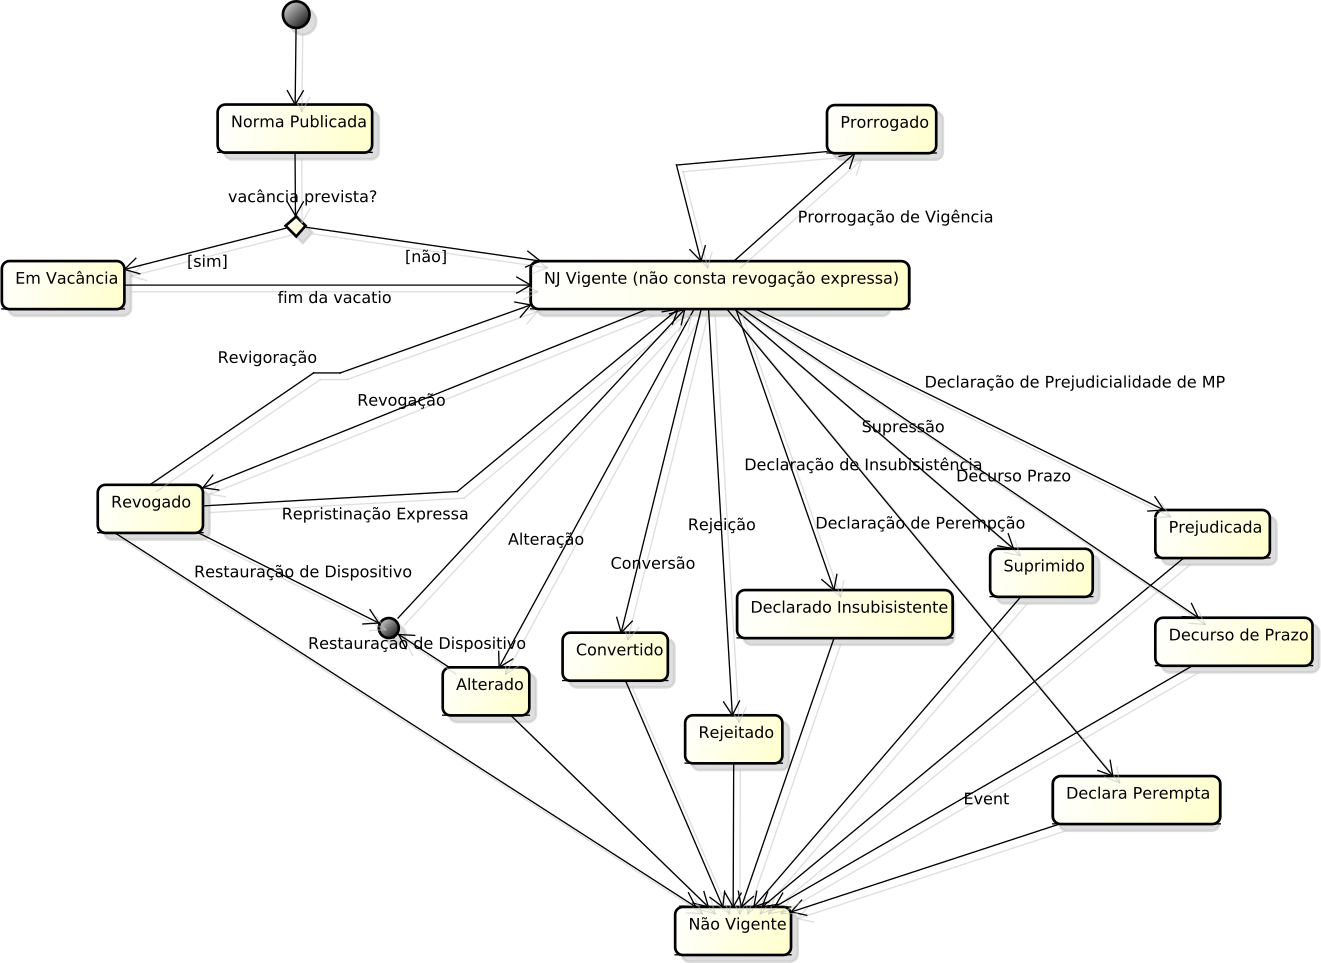
\includegraphics[scale=0.4]{Vigencia.pdf}
	\end{center}
	%\legend{Fonte: }
\end{figure}
% ---

% ---
\begin{figure}[htb]
	\caption{\label{fig_grafico_eficacia}Diagrama de Eficácia}
	\begin{center}
	    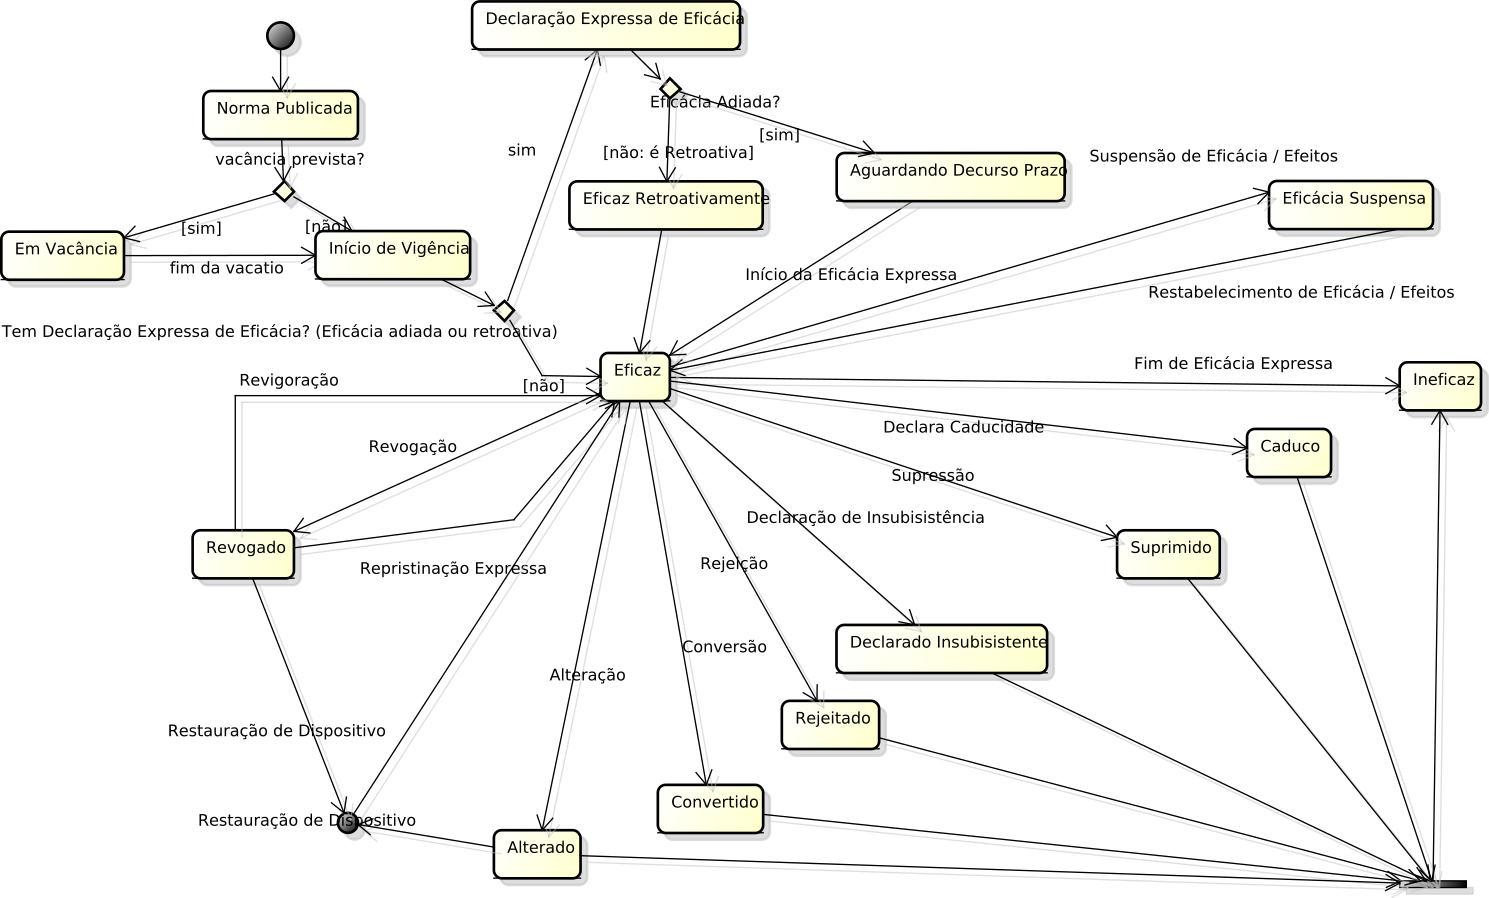
\includegraphics[scale=0.4]{Eficacia.pdf}
	\end{center}
	%\legend{Fonte: }
\end{figure}
% ---

% ---
\begin{figure}[htb]
	\caption{\label{fig_grafico_validade}Diagrama de Validade}
	\begin{center}
	    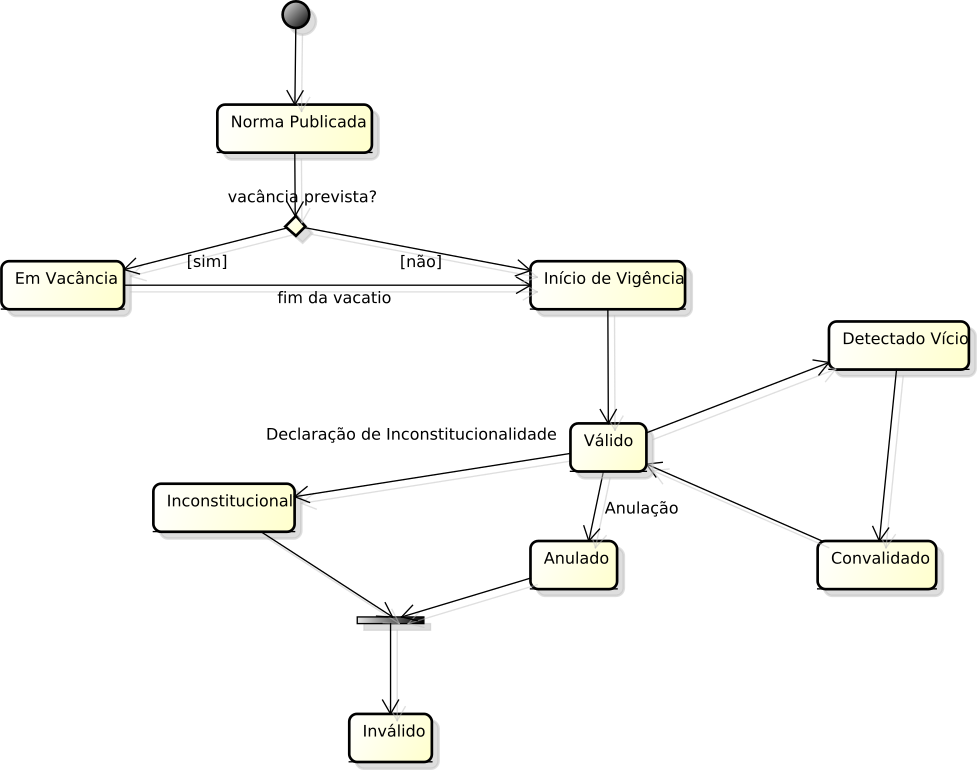
\includegraphics[scale=0.4]{Validade.pdf}
	\end{center}
	%\legend{Fonte: }
\end{figure}
% ---

% ---
\begin{figure}[htb]
	\caption{\label{fig_grafico_estagios-mp}Diagrama de Estágios da Medida
	Provisória}
	\begin{center}
	    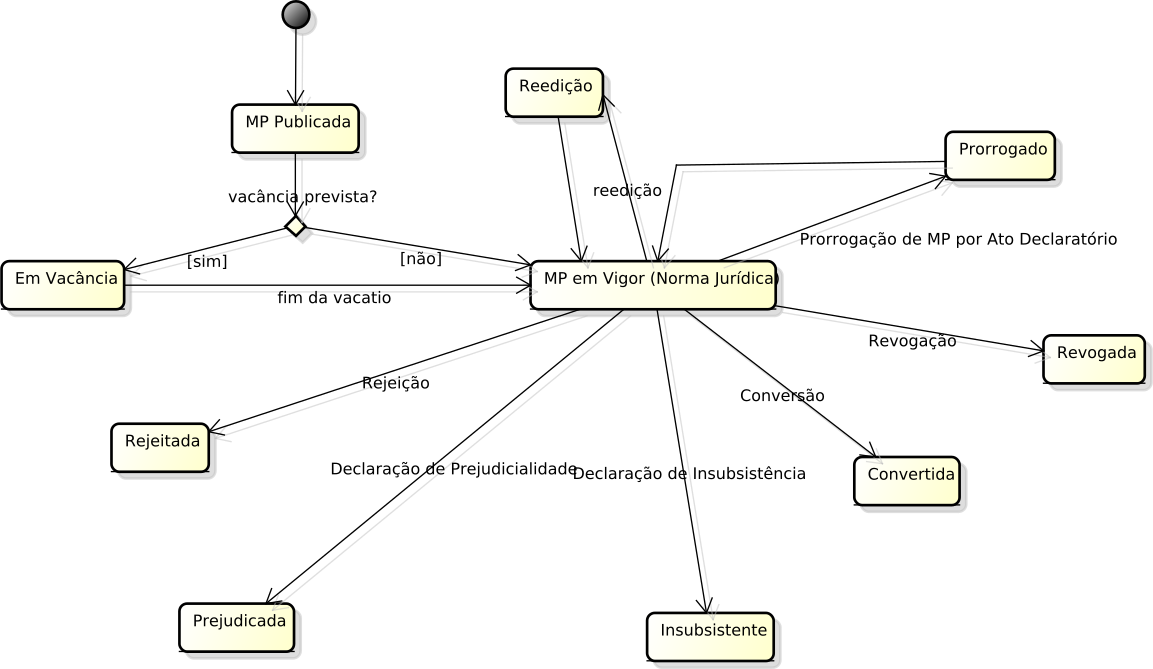
\includegraphics[scale=0.4]{EstagiosMP.pdf}
	\end{center}
	%\legend{Fonte: }
\end{figure}
% ---

% ---
\begin{figure}[htb]
	\caption{\label{fig_grafico_publicacao}Diagrama de Publicação}
	\begin{center}
	    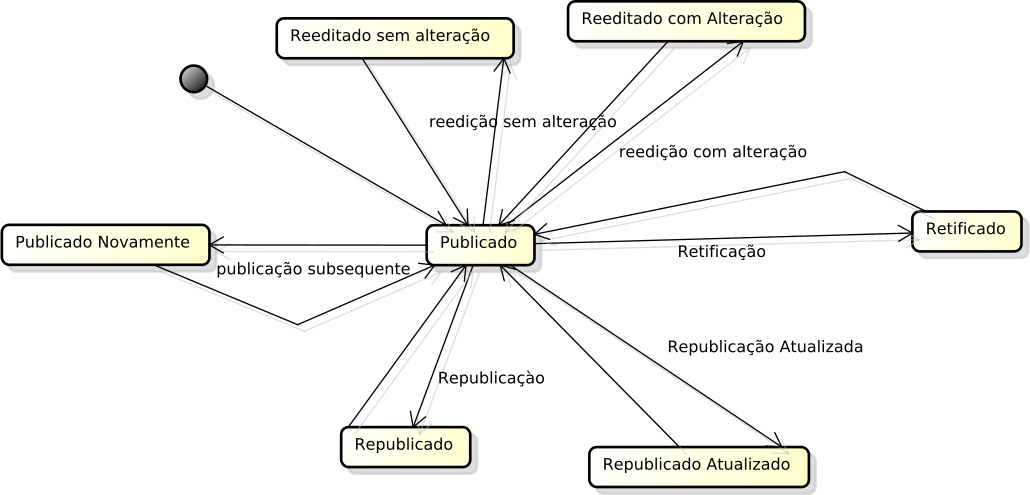
\includegraphics[scale=0.4]{Publicacao.pdf}
	\end{center}
	%\legend{Fonte: }
\end{figure}
% ---

% ---

\end{apendicesenv}
% ---

% ---
% Mesa Diretora
% ---

\cleardoublepage
\pagestyle{empty}
\newpage \mbox{}
\clearpage

\phantomsection
\pdfbookmark[0]{Mesa Diretora}{Mesa Diretora}
% \addcontentsline{toc}{chapter}{Mesa Diretora}

\vspace*{\fill}
{
\centering
\setlength{\parindent}{0cm}
\setlength{\parskip}{0.5cm}  % tente também \onelineskip

\ABNTEXchapterfont

{
\large
\textbf{SENADO FEDERAL}\\
Mesa\\
Biênio 2013 -- 2014\\
}

\vspace*{\parskip}
Senador Renan Calheiros\\
\textbf{PRESIDENTE}\\

% first column

\begin{multicols}{2}

Senador Jorge Viana\\
\textbf{PRIMEIRO-VICE-PRESIDENTE}

Senador Romero Jucá\\
\textbf{SEGUNDO-VICE-PRESIDENTE}

Senador Flexa Ribeiro\\
\textbf{PRIMEIRO-SECRETÁRIO}

%second column
\columnbreak

Senadora Ângela Portela\\
\textbf{SEGUNDA-SECRETÁRIA}

Senador Ciro Nogueira\\
\textbf{TERCEIRO-SECRETÁRIO}

Senador João Vicente Claudino\\
\textbf{QUARTO-SECRETÁRIO}

\end{multicols}

Senador Magno Malta\\
\textbf{PRIMEIRO-SUPLENTE}

Senador Jayme Campos\\
\textbf{SEGUNDO-SUPLENTE}

Senador João Durval\\
\textbf{TERCEIRO-SUPLENTE}

Senador Casildo Maldaner\\
\textbf{QUARTO-SUPLENTE}

\rule{5cm}{\ABNTEXsignthickness}%

Doris Peixoto\\
\textbf{DIRETORA-GERAL}

Claudia Lyra\\
\textbf{SECRETÁRIA-GERAL DA MESA}

}
\vspace*{\fill}


%---------------------------------------------------------------------
% INDICE REMISSIVO
%---------------------------------------------------------------------
% \printindex

\end{document}
